\documentclass[../../../main]{subfiles}
\begin{document}

\section{結果}\label{sec:result}

\subsection{実験1の結果}
実験1で撮影したオシロスコープの波形を図\ref{fig:oscilloscope-raw}に示す。
この図をもとに、波形を抽出したものを図\ref{fig:oscilloscope-each}に示す。

\clearpage
\subsection{実験2の結果}
実験2で撮影したオシロスコープの波形は図\ref{fig:time-constant}に示す。
この図から$t=T$、すなわちゲインの$1-e^{-1}\approx63.2\%$となる時刻を読み取ると、
\SI{95}{\milli\sec}、\SI{98}{\milli\sec}、\SI{95}{\milli\sec}であった。
これらを平均して、$T = \SI{96}{\milli\sec}$と得られた。

\clearpage
\subsection{実験3の結果}
実験3で測定した、あるPゲインに対する$e$、$e_p$の値、
$e_p = k_p e$より計算される$k_p$の値を次の表\ref{tab:e-ep}に示す。
\begin{table}[!ht]
	\centering
	\caption{Pゲインに対する$e$、$e_p$の値と計算される$k_p$の値}\label{tab:e-ep}
	\begin{tabular}{cccc}
		\hline
		$P$ & $e$              & $e_p$       & $k_p$           \\ \hline
		60  & 0.9              & 8.6         & 9.5             \\
		60  & 0.6              & 6.8         & 11              \\
		60  & -1.0             & -7.5        & 7.5             \\
		60  & -1.2             & -9.0        & 7.5             \\
		80  & -0.8             & -8.5        & 10              \\
		80  & -0.6             & -5.6        & 9.3             \\
		80  & 0.40             & 6.5         & 16.2            \\
		80  & 0.65             & 8.7         & 13              \\
		100 & \SI{-3.40E-02}{} & \SI{-5.7}{} & \SI{1.7E+02}{}  \\
		100 & \SI{-2.75E-02}{} & \SI{-4.2}{} & \SI{1.5E+02} {} \\
		100 & \SI{2.38E-02}{}  & \SI{6.7}{}  & \SI{2.8E+02}{}  \\
		100 & \SI{3.40E-02}{}  & \SI{ 8.9}{} & \SI{2.6E+02}{}  \\ \hline
	\end{tabular}
\end{table}

この値をもとに$P$に対する$e$、$e_p$の関係を\ref{fig:e-e_p-relation}に示す。
それぞれ原点を通る直線で近似したものと、一次関数で近似したものを示している。
ここでは、得られた実験値に近いものとして、
$P=60$のとき、$e_p = 8.58e + 1.23$、
$P-80$のとき、$e_p = 11.93e + 1.32$、
$P=100$のとき、$e_p = 213.97e + 1.62$
とする。
\begin{figure}
	\centering
	\begin{subfigure}{0.45\linewidth}
		\centering
		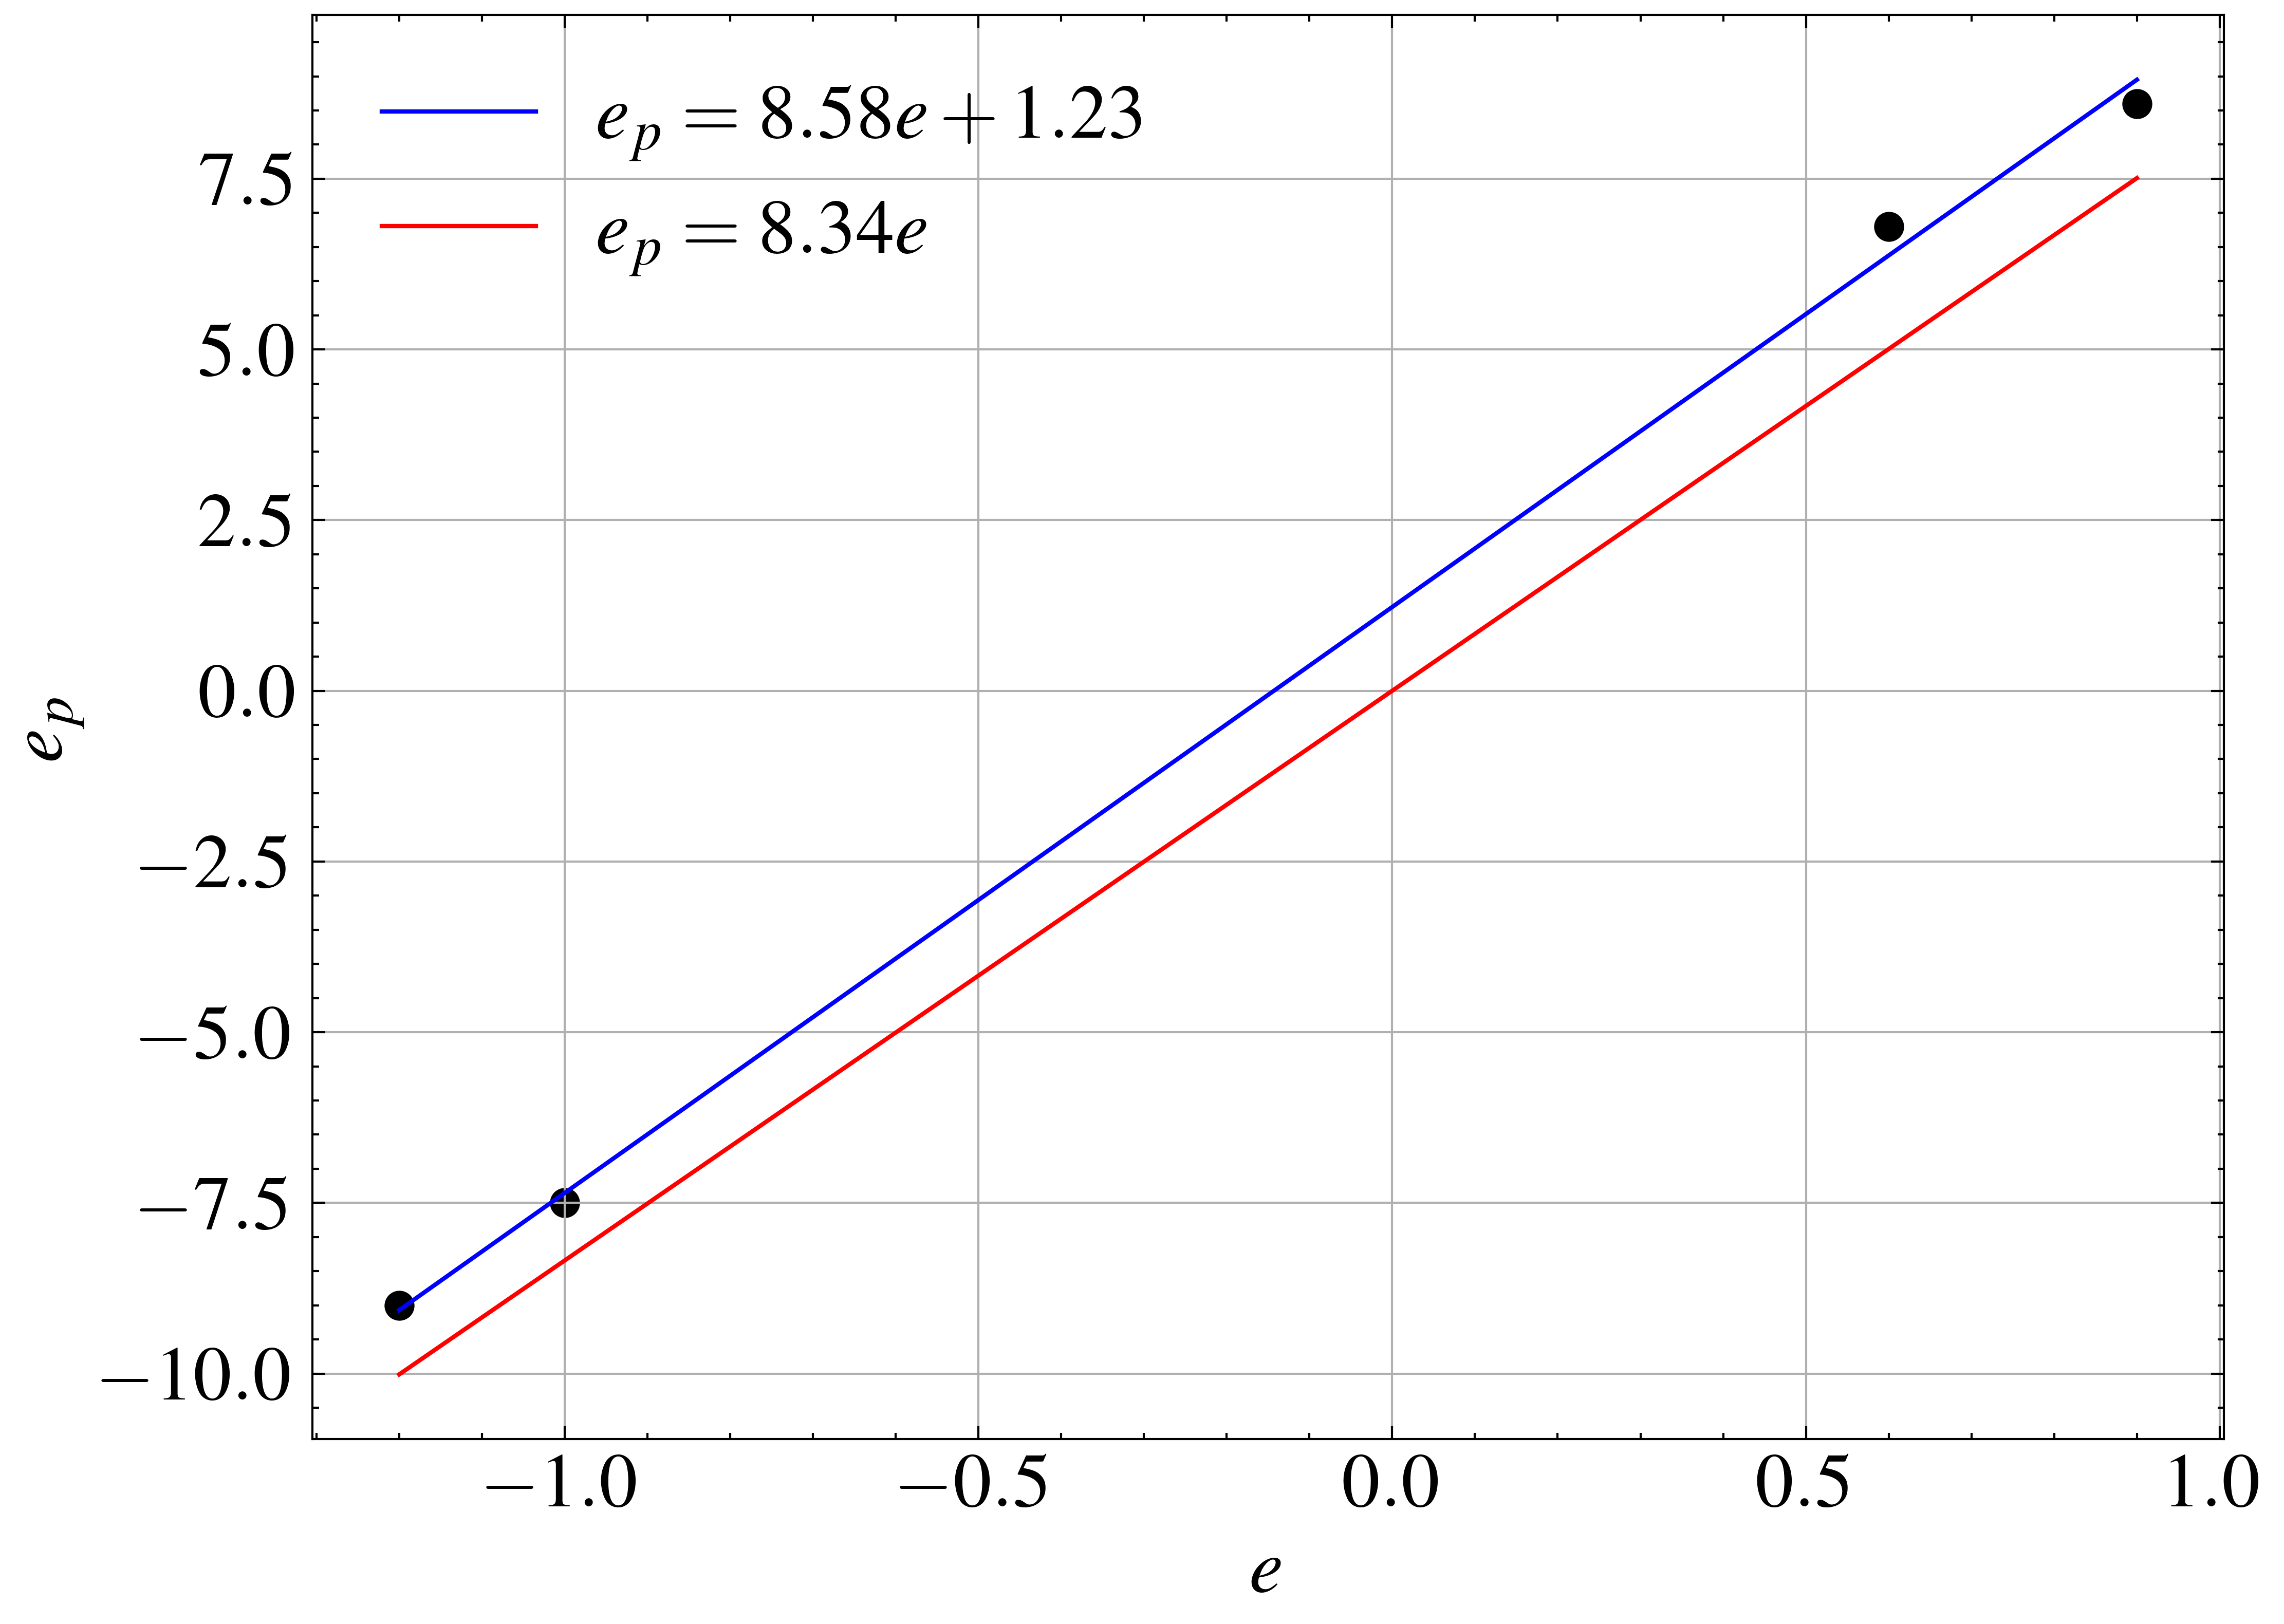
\includegraphics[width=\linewidth]{src/figures/e-e_p-relation/e-e_p-relation-60.png}
		\subcaption{$P=60$}\label{fig:e-e_p-relation-60}
	\end{subfigure}
	\begin{subfigure}{0.45\linewidth}
		\centering
		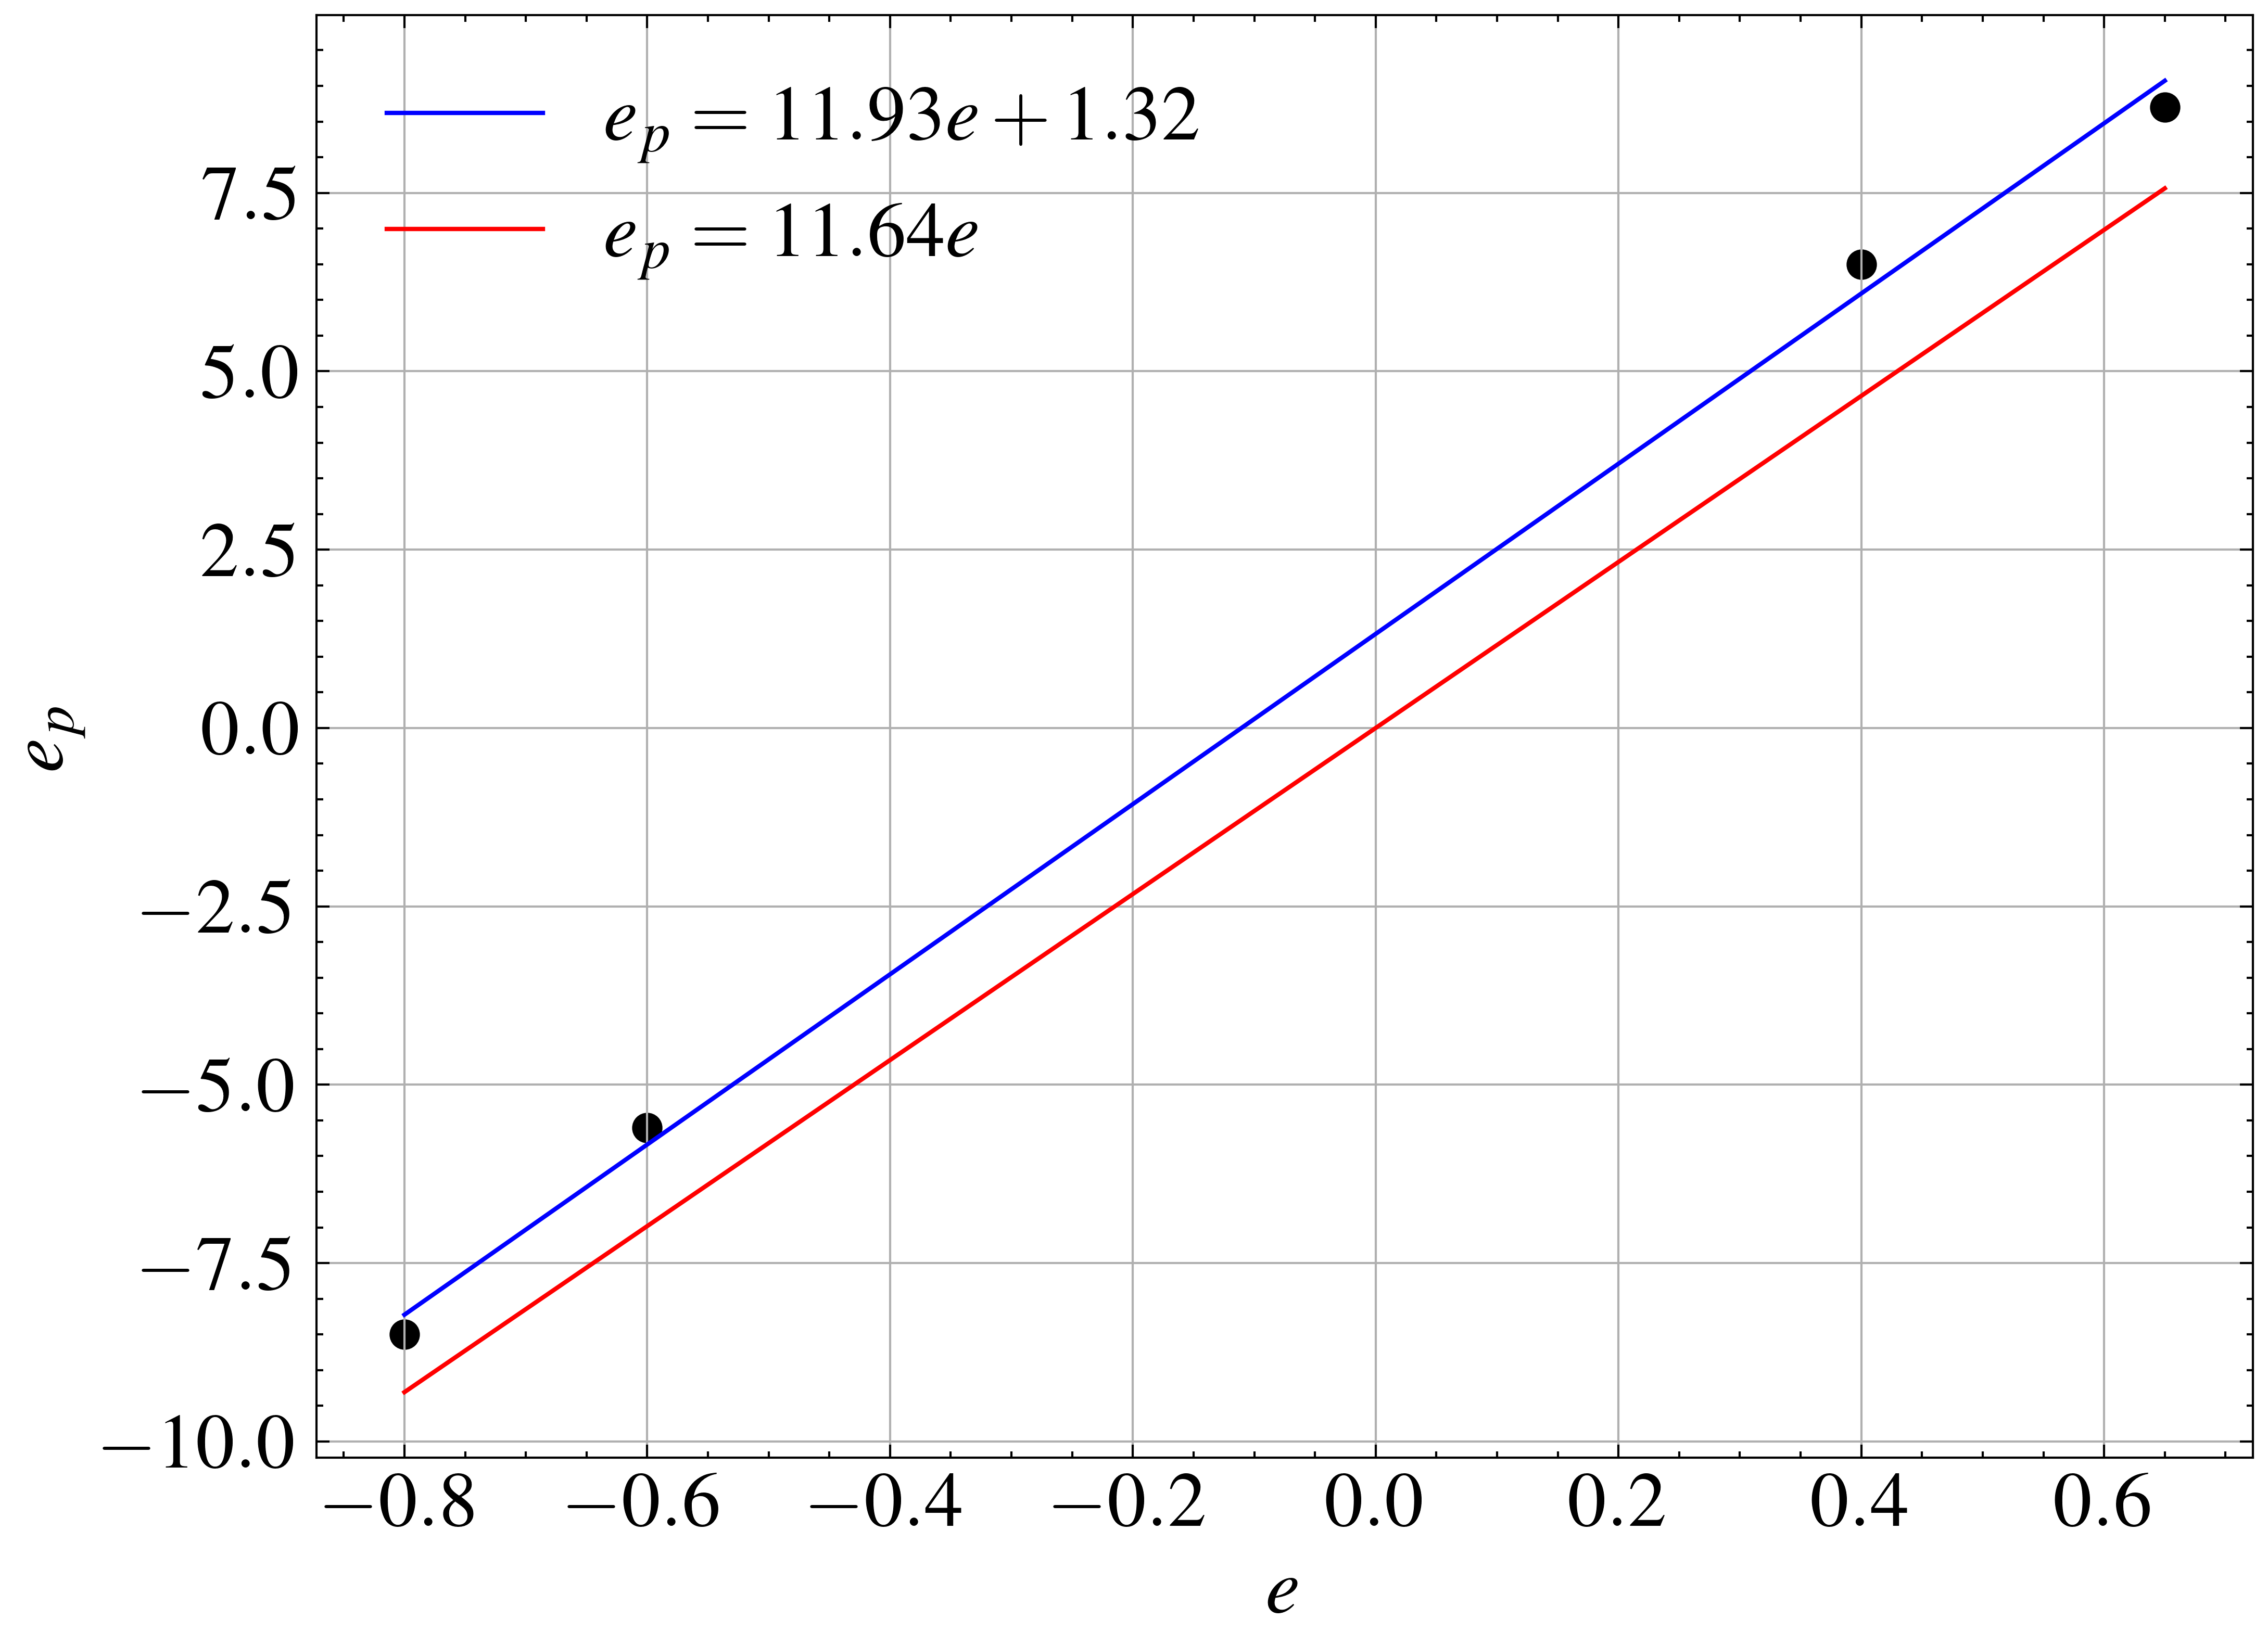
\includegraphics[width=\linewidth]{src/figures/e-e_p-relation/e-e_p-relation-80.png}
		\subcaption{$P=80$}\label{fig:e-e_p-relation-80}
	\end{subfigure}
	\begin{subfigure}{0.45\linewidth}
		\centering
		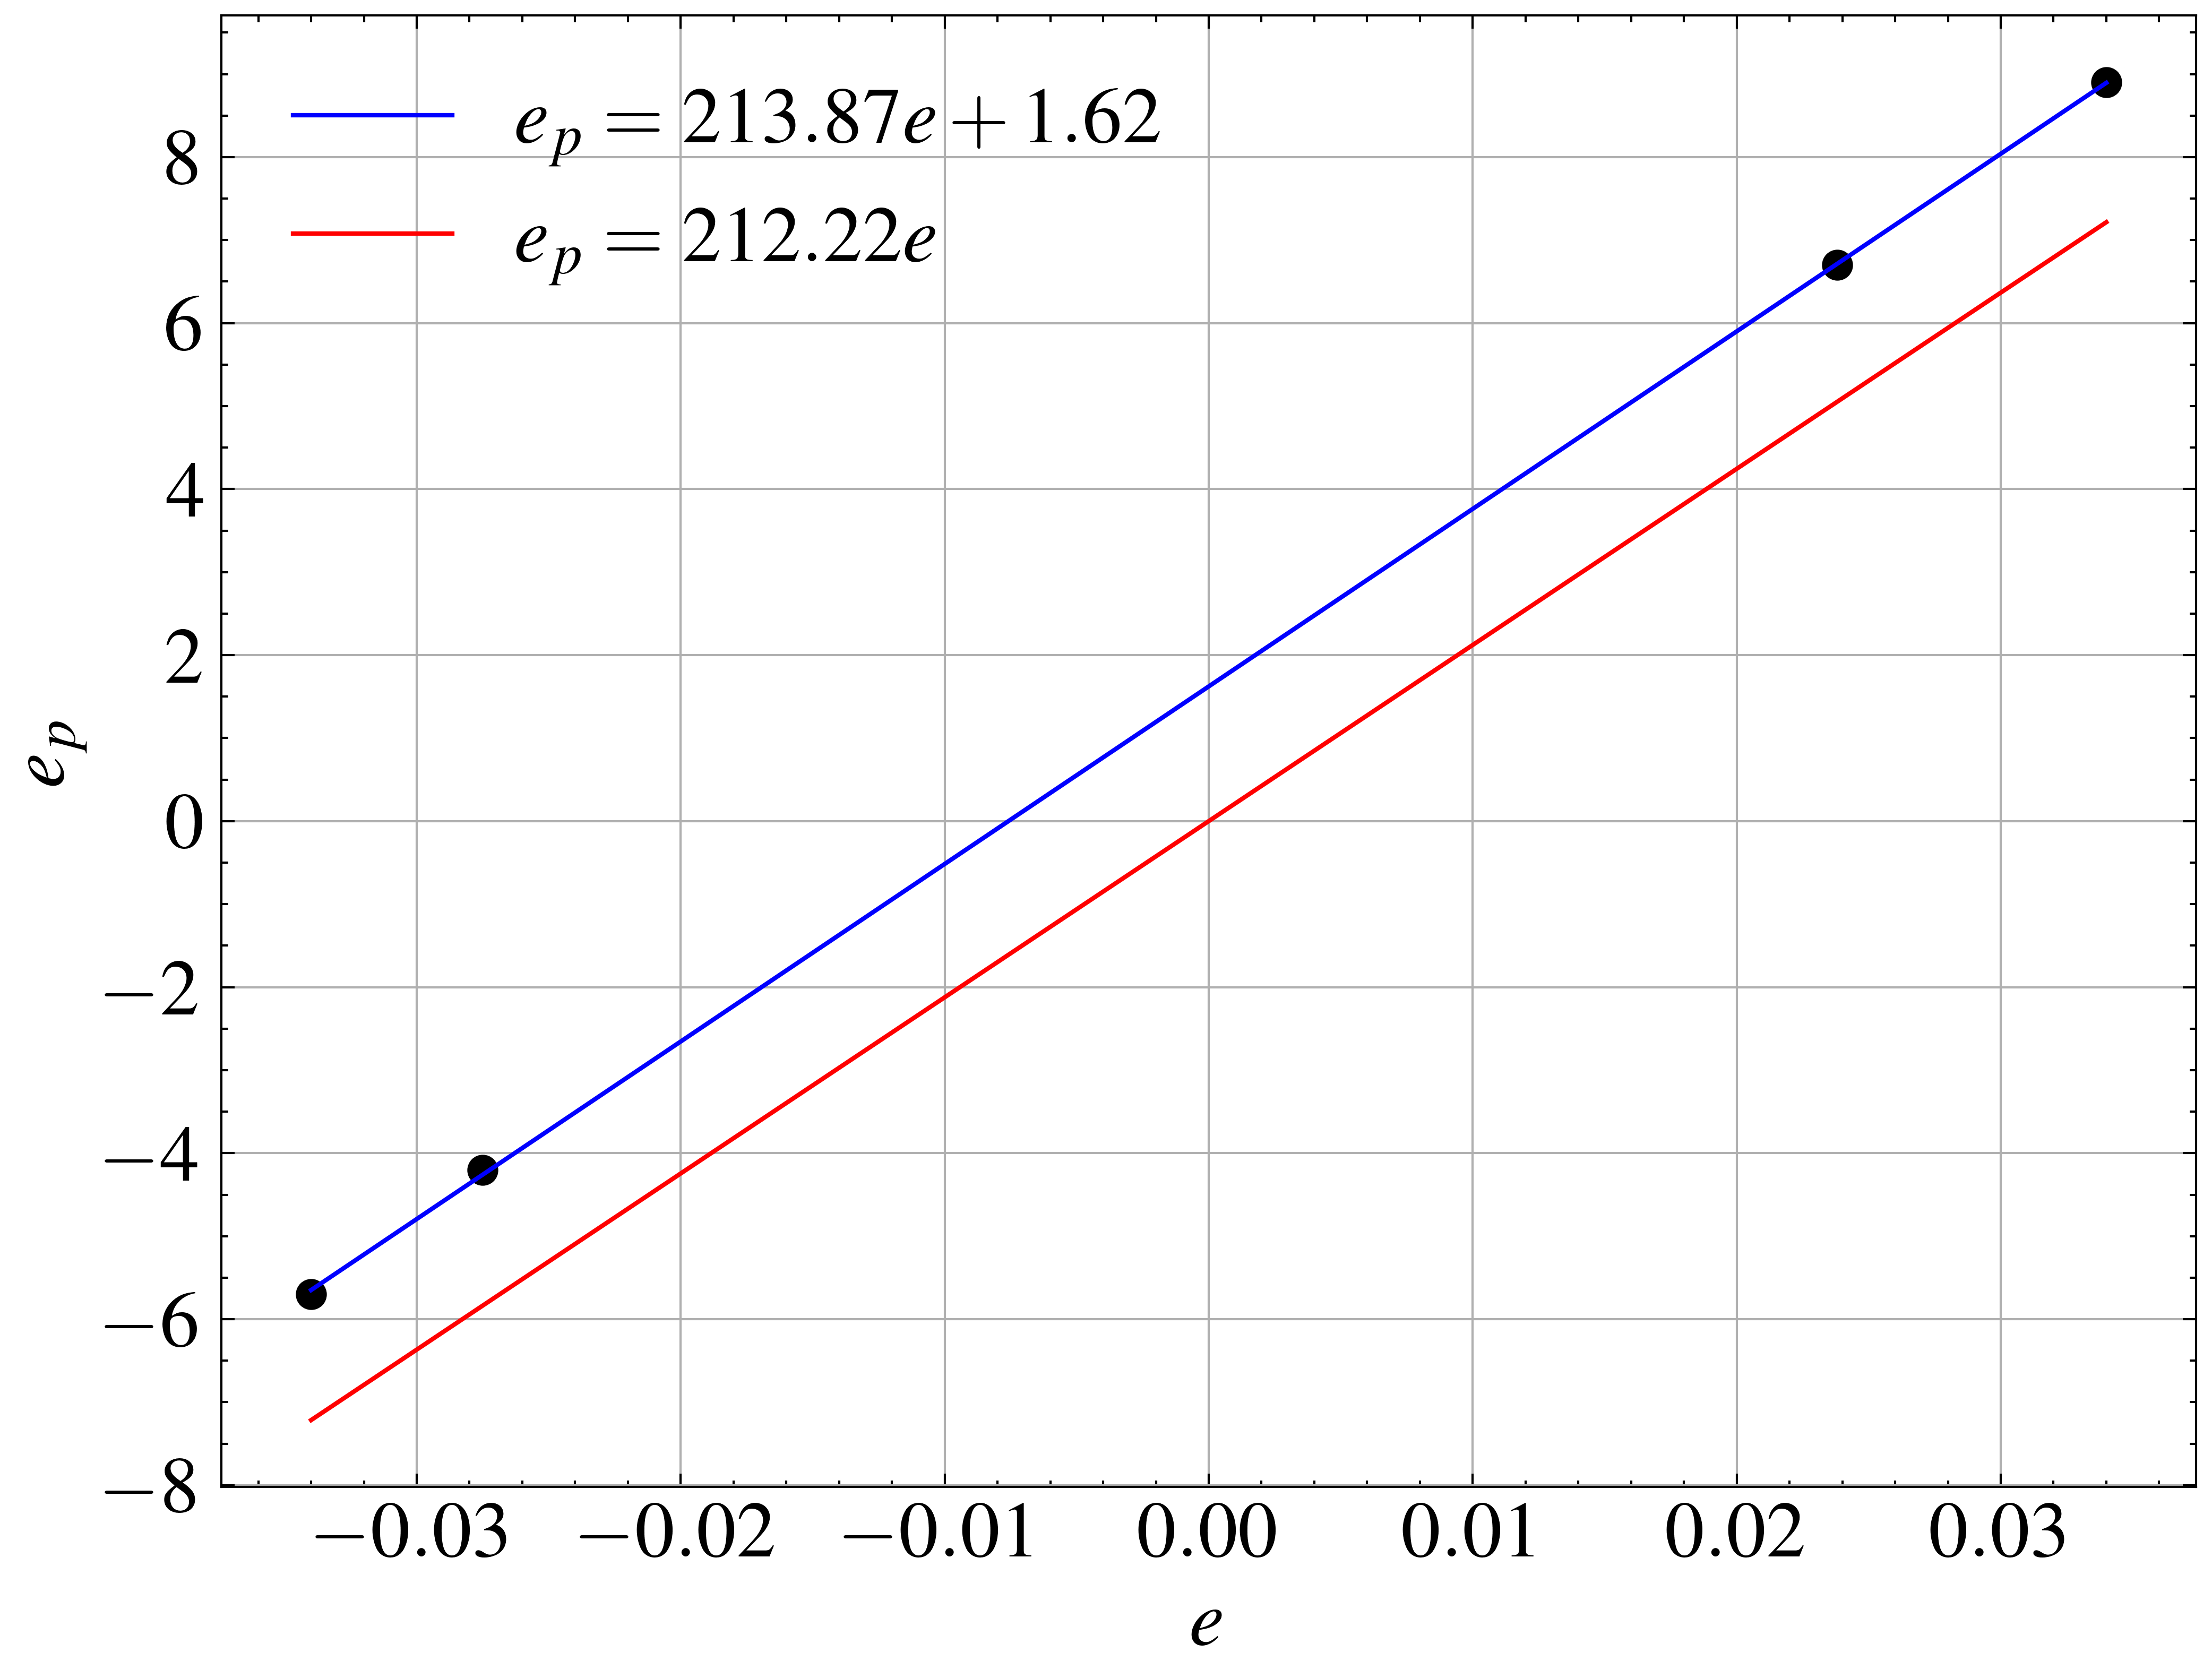
\includegraphics[width=\linewidth]{src/figures/e-e_p-relation/e-e_p-relation-100.png}
		\subcaption{$P=100$}\label{fig:e-e_p-relation-100}
	\end{subfigure}

	\caption{$e$と$e_p$の関係}\label{fig:e-e_p-relation}
\end{figure}


さらに、$P$に対する$e_p$と計測した$\dot{\theta_2}$の関係を表\ref{tab:theta_dot-e_p-relation}に示す。
なお、$\Xi_2$は計測時、回転体についていた4つの印を回転速度系にて計測した値であり、
$\dot{\theta_2} = \Xi_2 \dfrac{2\pi}{60}$の関係にある。
また、$K$は定常状態において、$\dot{\theta_2} = K e_p$の関係にあり、\si{\radian\per\sec\per\volt}の単位を持つ。
\begin{table}[!ht]
    \centering
    \caption{$P$に対する$e_p$と$\dot{\theta_2}$の関係}\label{tab:theta_dot-e_p-relation}
    \begin{tabular}{cccccc}
        \hline
        $P$ & $e_p$ / \si{\volt} & $\Xi_2$ /rpm & $\dot{\theta_2}$ / \si{\radian\per\sec} & $K$ \si{\radian\per\sec\per\volt} \\ \hline
        60  & 8.6                & 280.0        & 7.330                                   & 0.8523                            \\
        60  & 6.8                & 180.4        & 4.722                                   & 0.6945                            \\
        60  & -7.5               & -263.5       & -6.898                                  & 0.9197                            \\
        60  & -9                 & -320.6       & -8.393                                  & 0.9325                            \\
        80  & -8.5               & -297.2       & -7.780                                  & 0.9153                            \\
        80  & -5.6               & -188.4       & -4.932                                  & 0.8807                            \\
        80  & 6.5                & 191.5        & 5.013                                   & 0.7713                            \\
        80  & 8.7                & 284.0        & 7.435                                   & 0.8546                            \\
        100 & -5.7               & -186.0       & -4.869                                  & 0.8542                            \\
        100 & -4.2               & -126.8       & -3.319                                  & 0.7903                            \\
        100 & 6.7                & 200.4        & 5.246                                   & 0.7830                            \\
        100 & 8.9                & 295.8        & 7.744                                   & 0.8701                            \\ \hline
    \end{tabular}
\end{table}

これをもとに、$P$に対する$e_p$と$\dot{\theta_2}$の関係を図\ref{fig:theta_dot-e_p-relation}に示す。
$e$と、$e_p$の関係と同様に、それぞれ原点を通る直線で近似したものと、一次関数で近似したものを示している。
$K$の値は表やグラフからもわかる様に$P$によってほぼ変わらず、
また、切片の値も小さいことから$\dot{\theta_2}=K e_p$とかけるする。
各$P$で平均をとって$K=\SI{0.85}{\radian\per\sec\per\volt}$とする。
\begin{figure}
	\centering
	\begin{subfigure}{0.48\columnwidth}
		\centering
		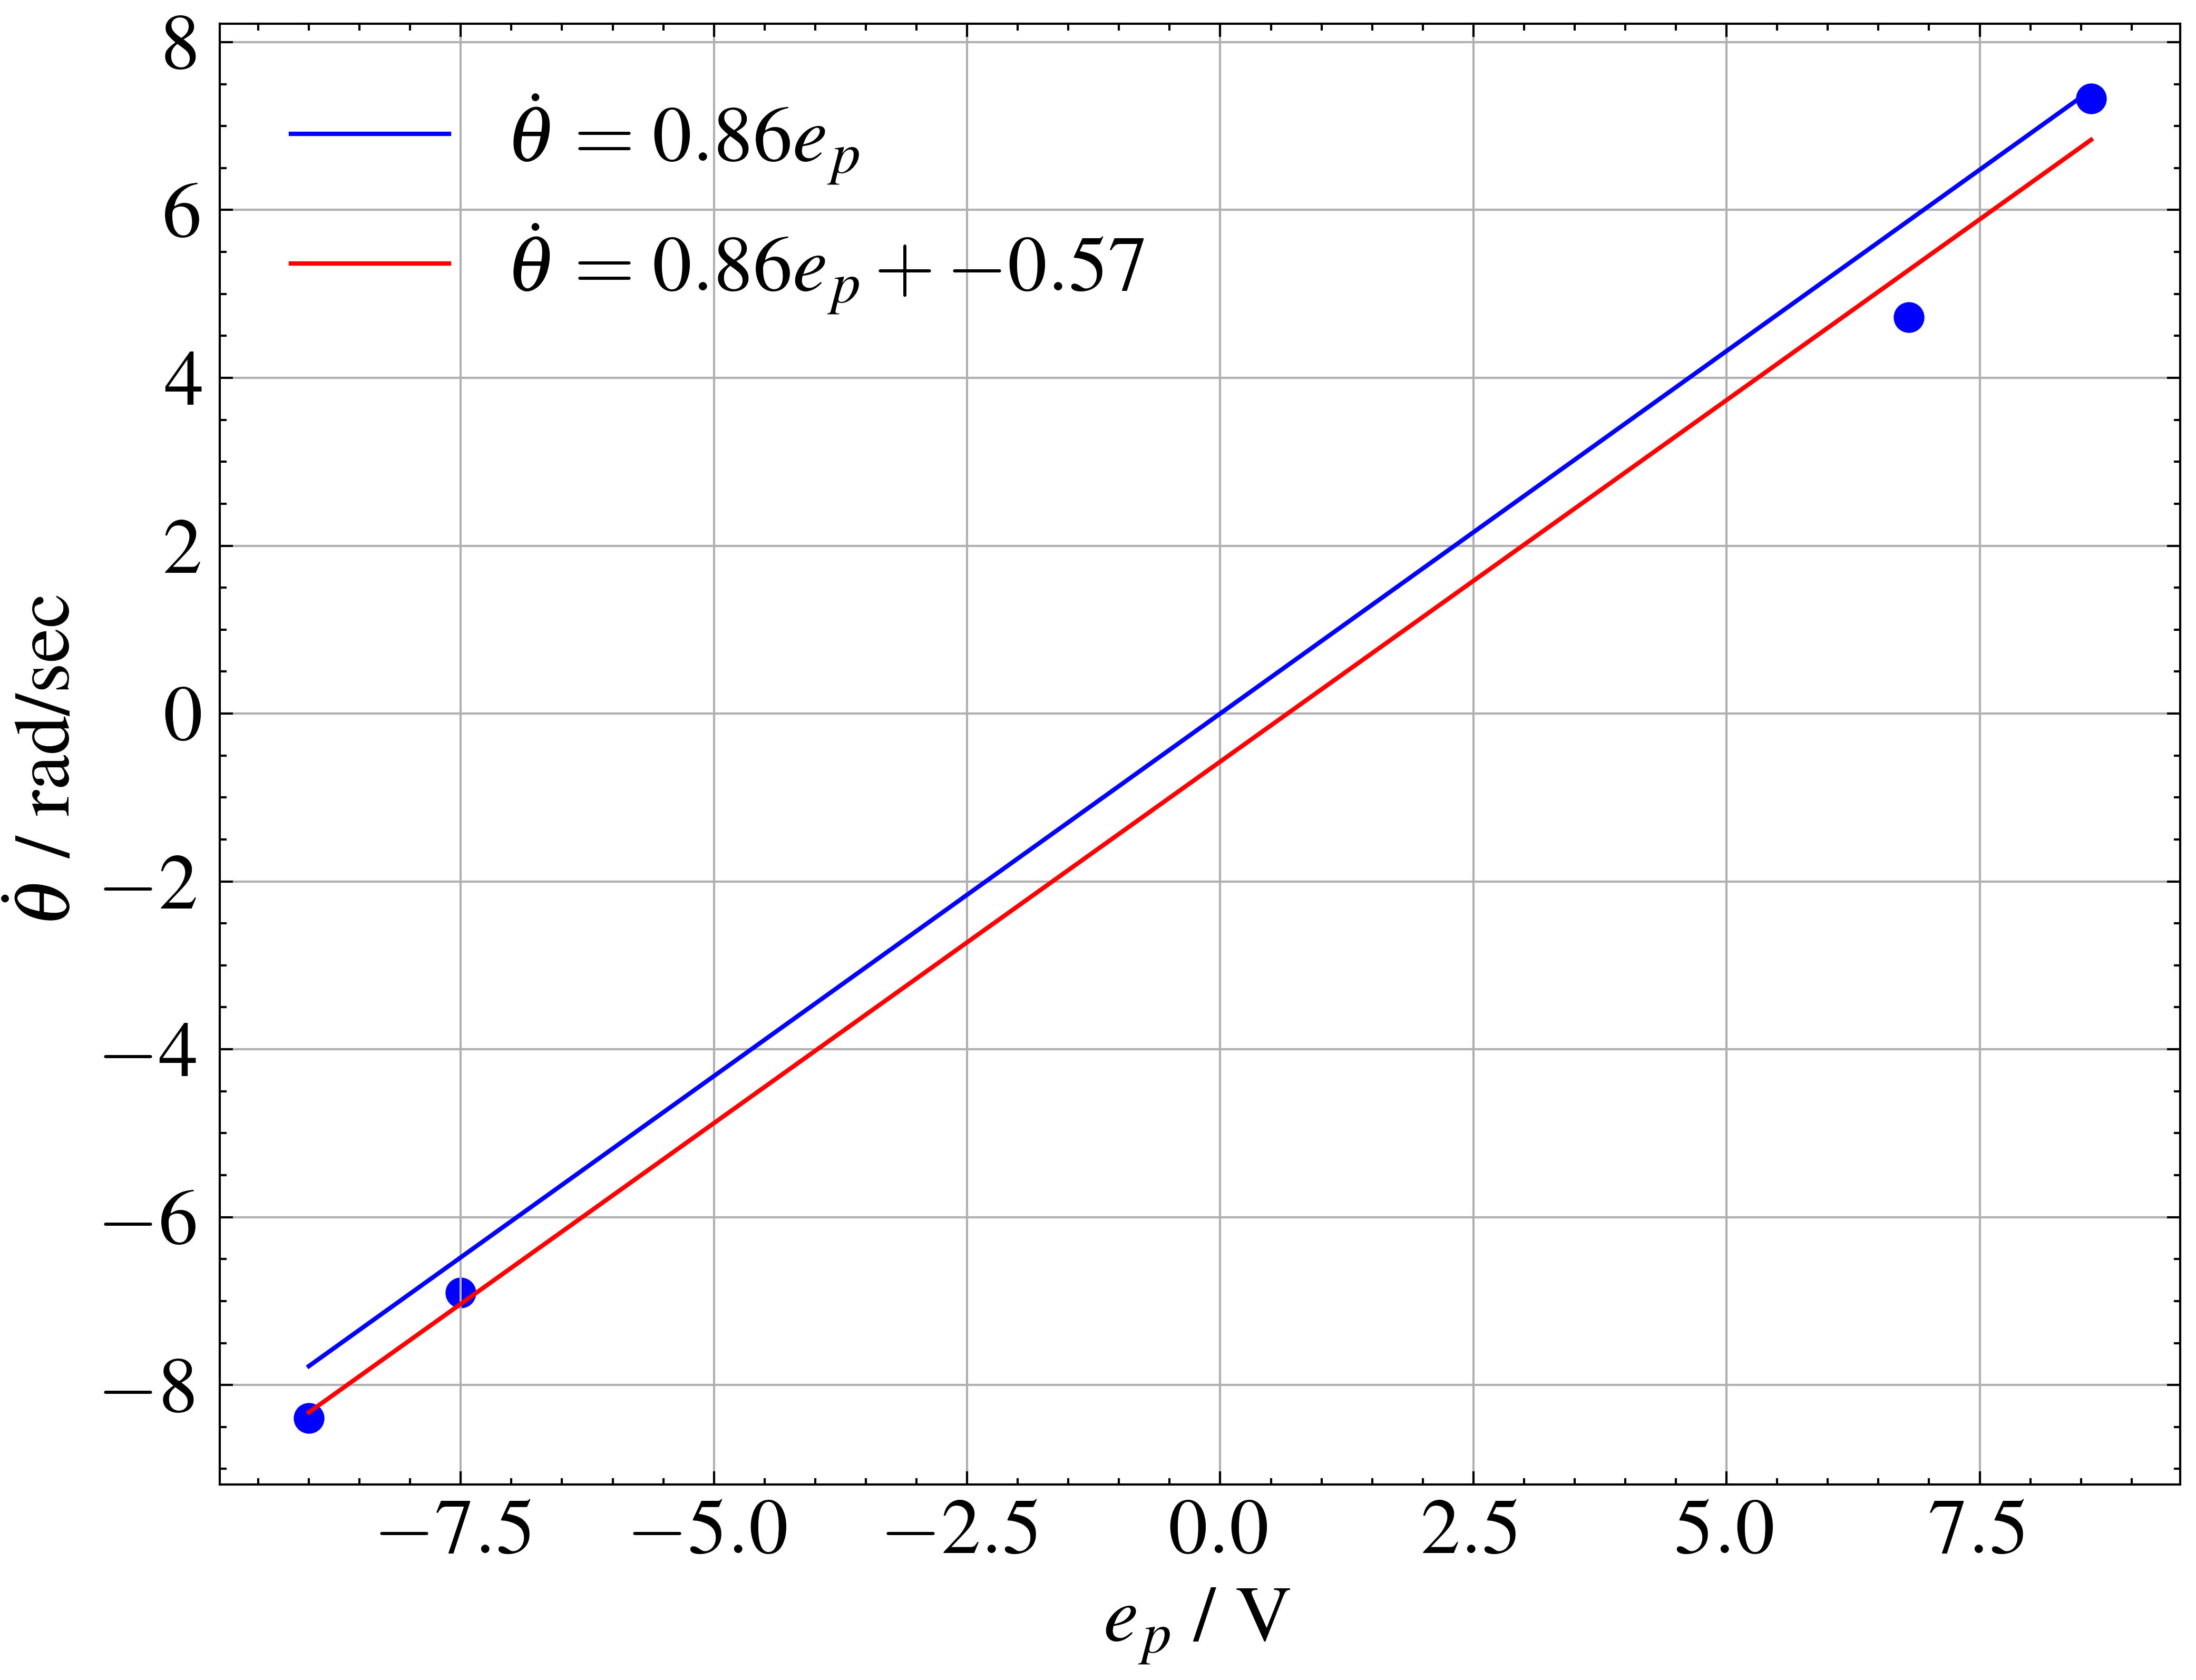
\includegraphics[width=0.8\linewidth]{src/figures/theta_dot-e_p-relation/theta_dot-e_p-relation-P60.png}
		\subcaption{$P=60$}
	\end{subfigure}
	\begin{subfigure}{0.48\columnwidth}
		\centering
		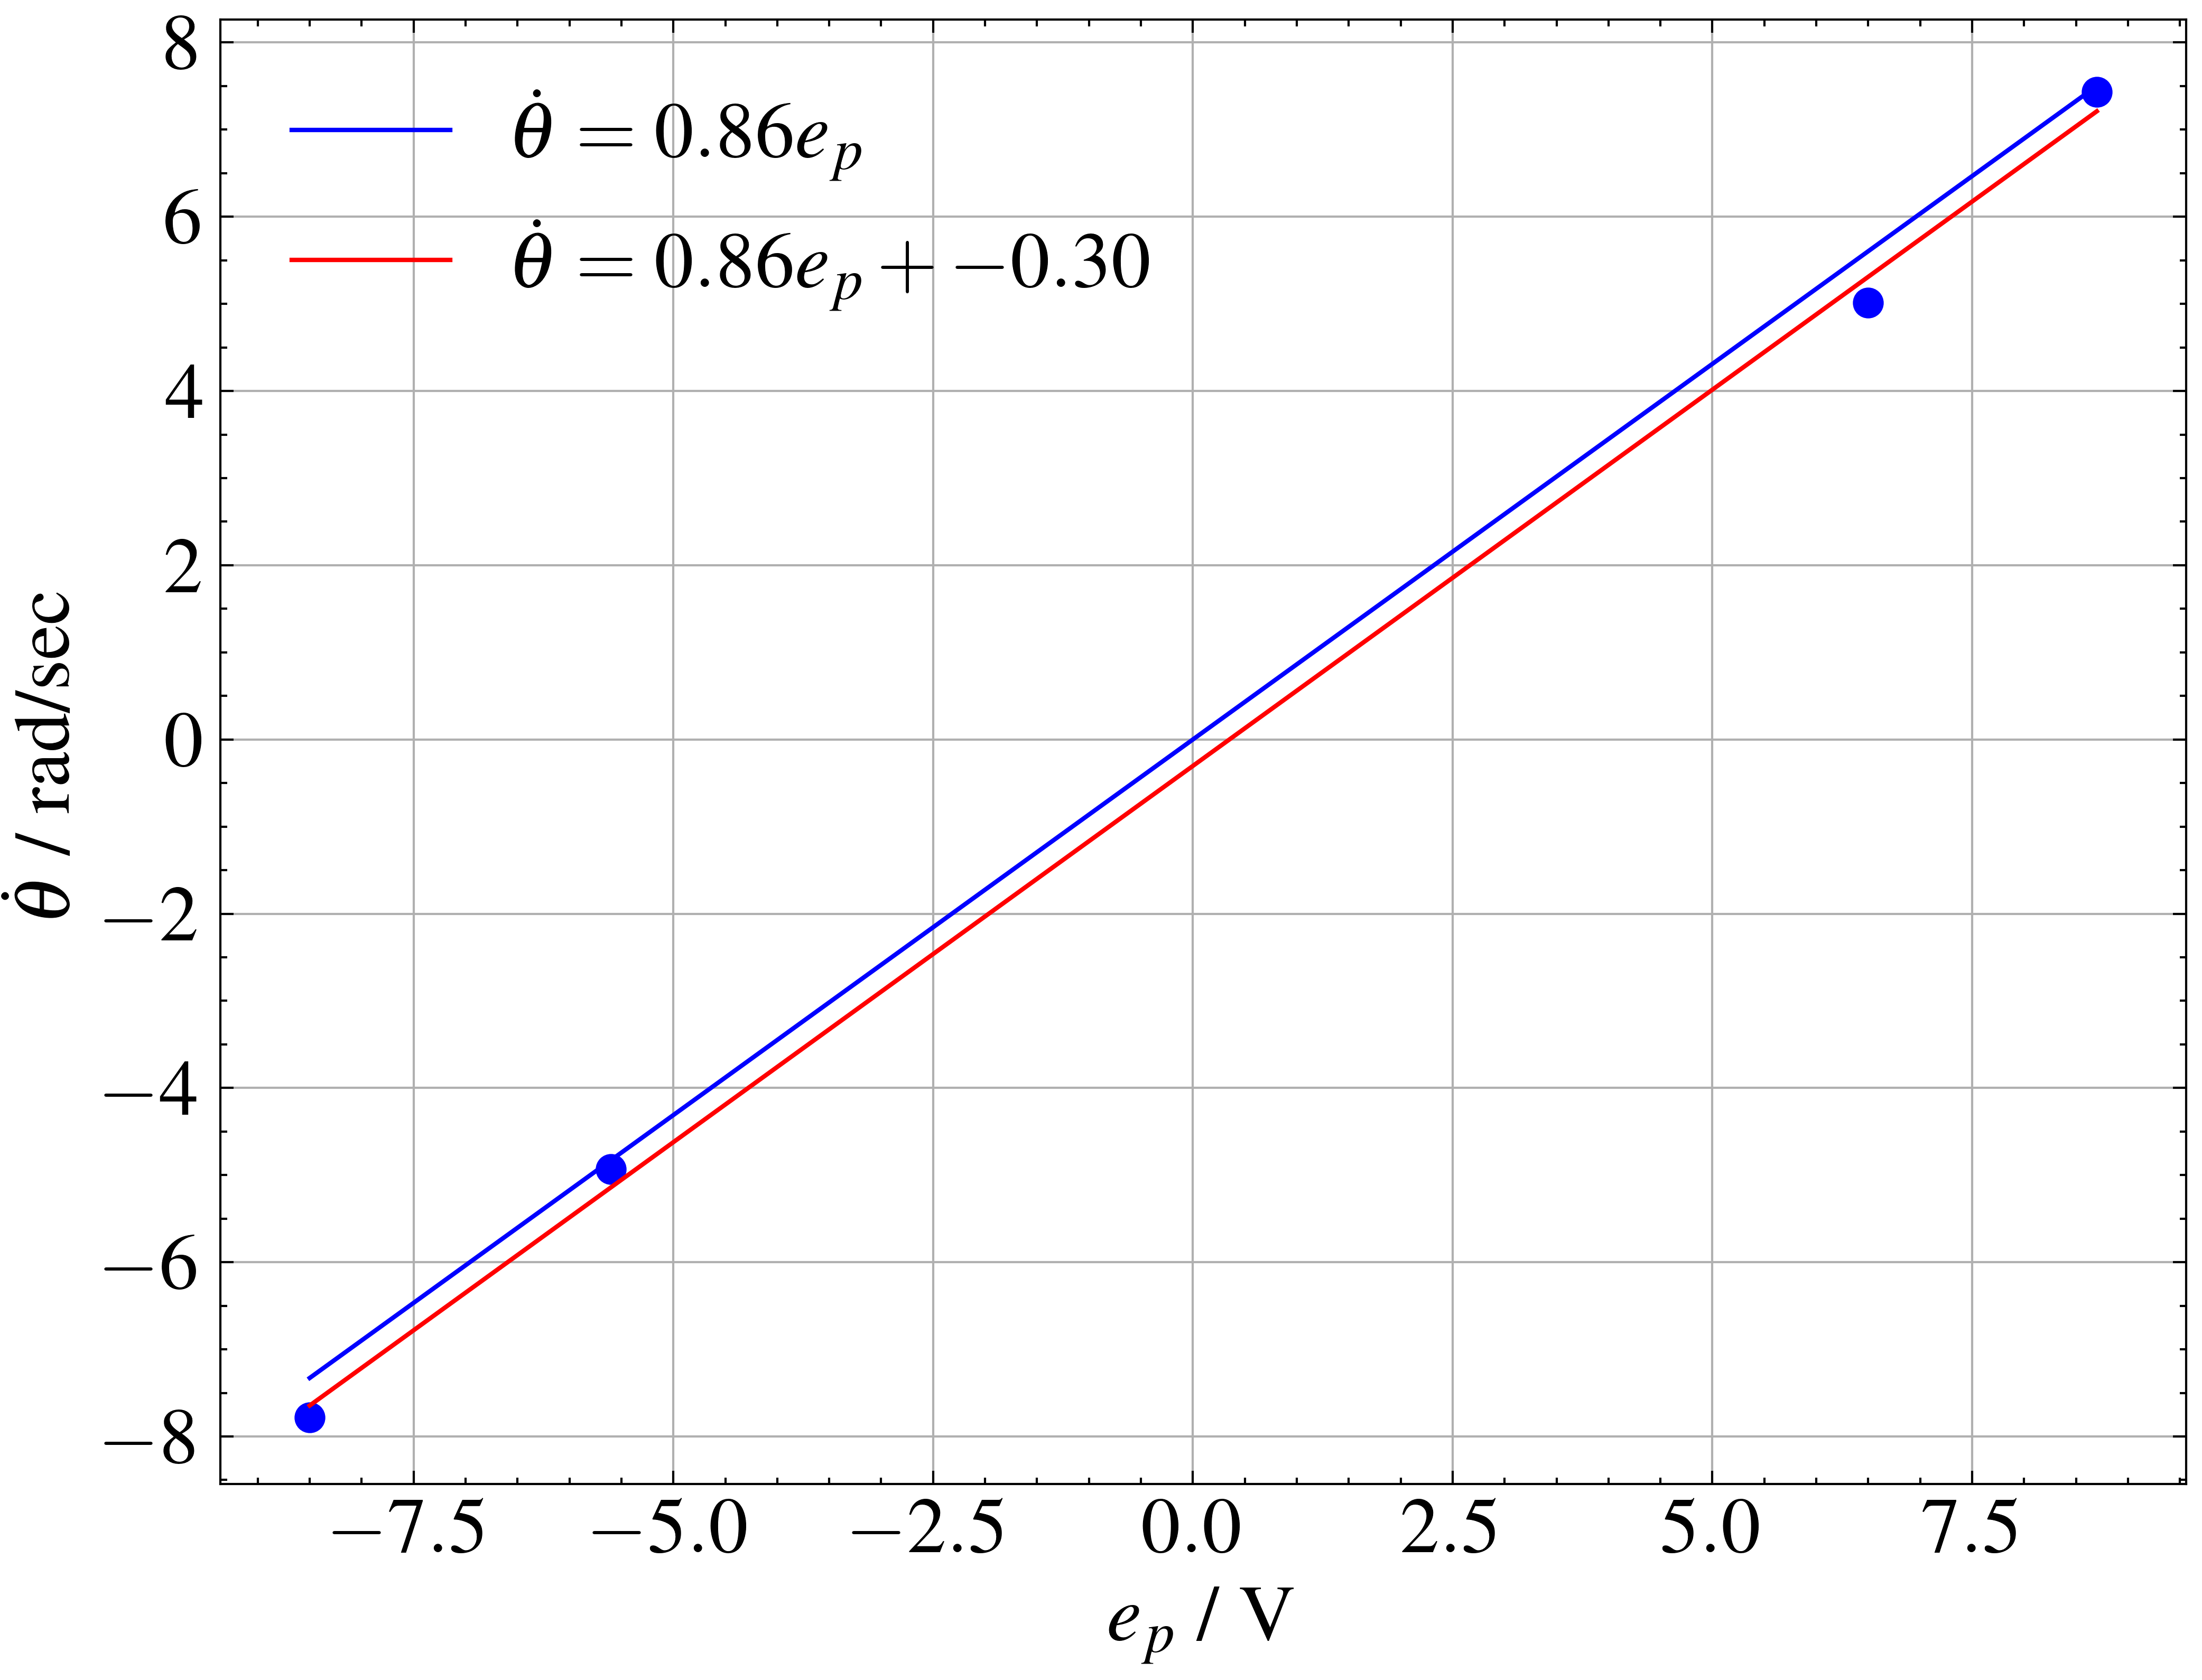
\includegraphics[width=0.8\linewidth]{src/figures/theta_dot-e_p-relation/theta_dot-e_p-relation-P80.png}
		\subcaption{$P=80$}
	\end{subfigure}
	\begin{subfigure}{0.48\columnwidth}
		\centering
		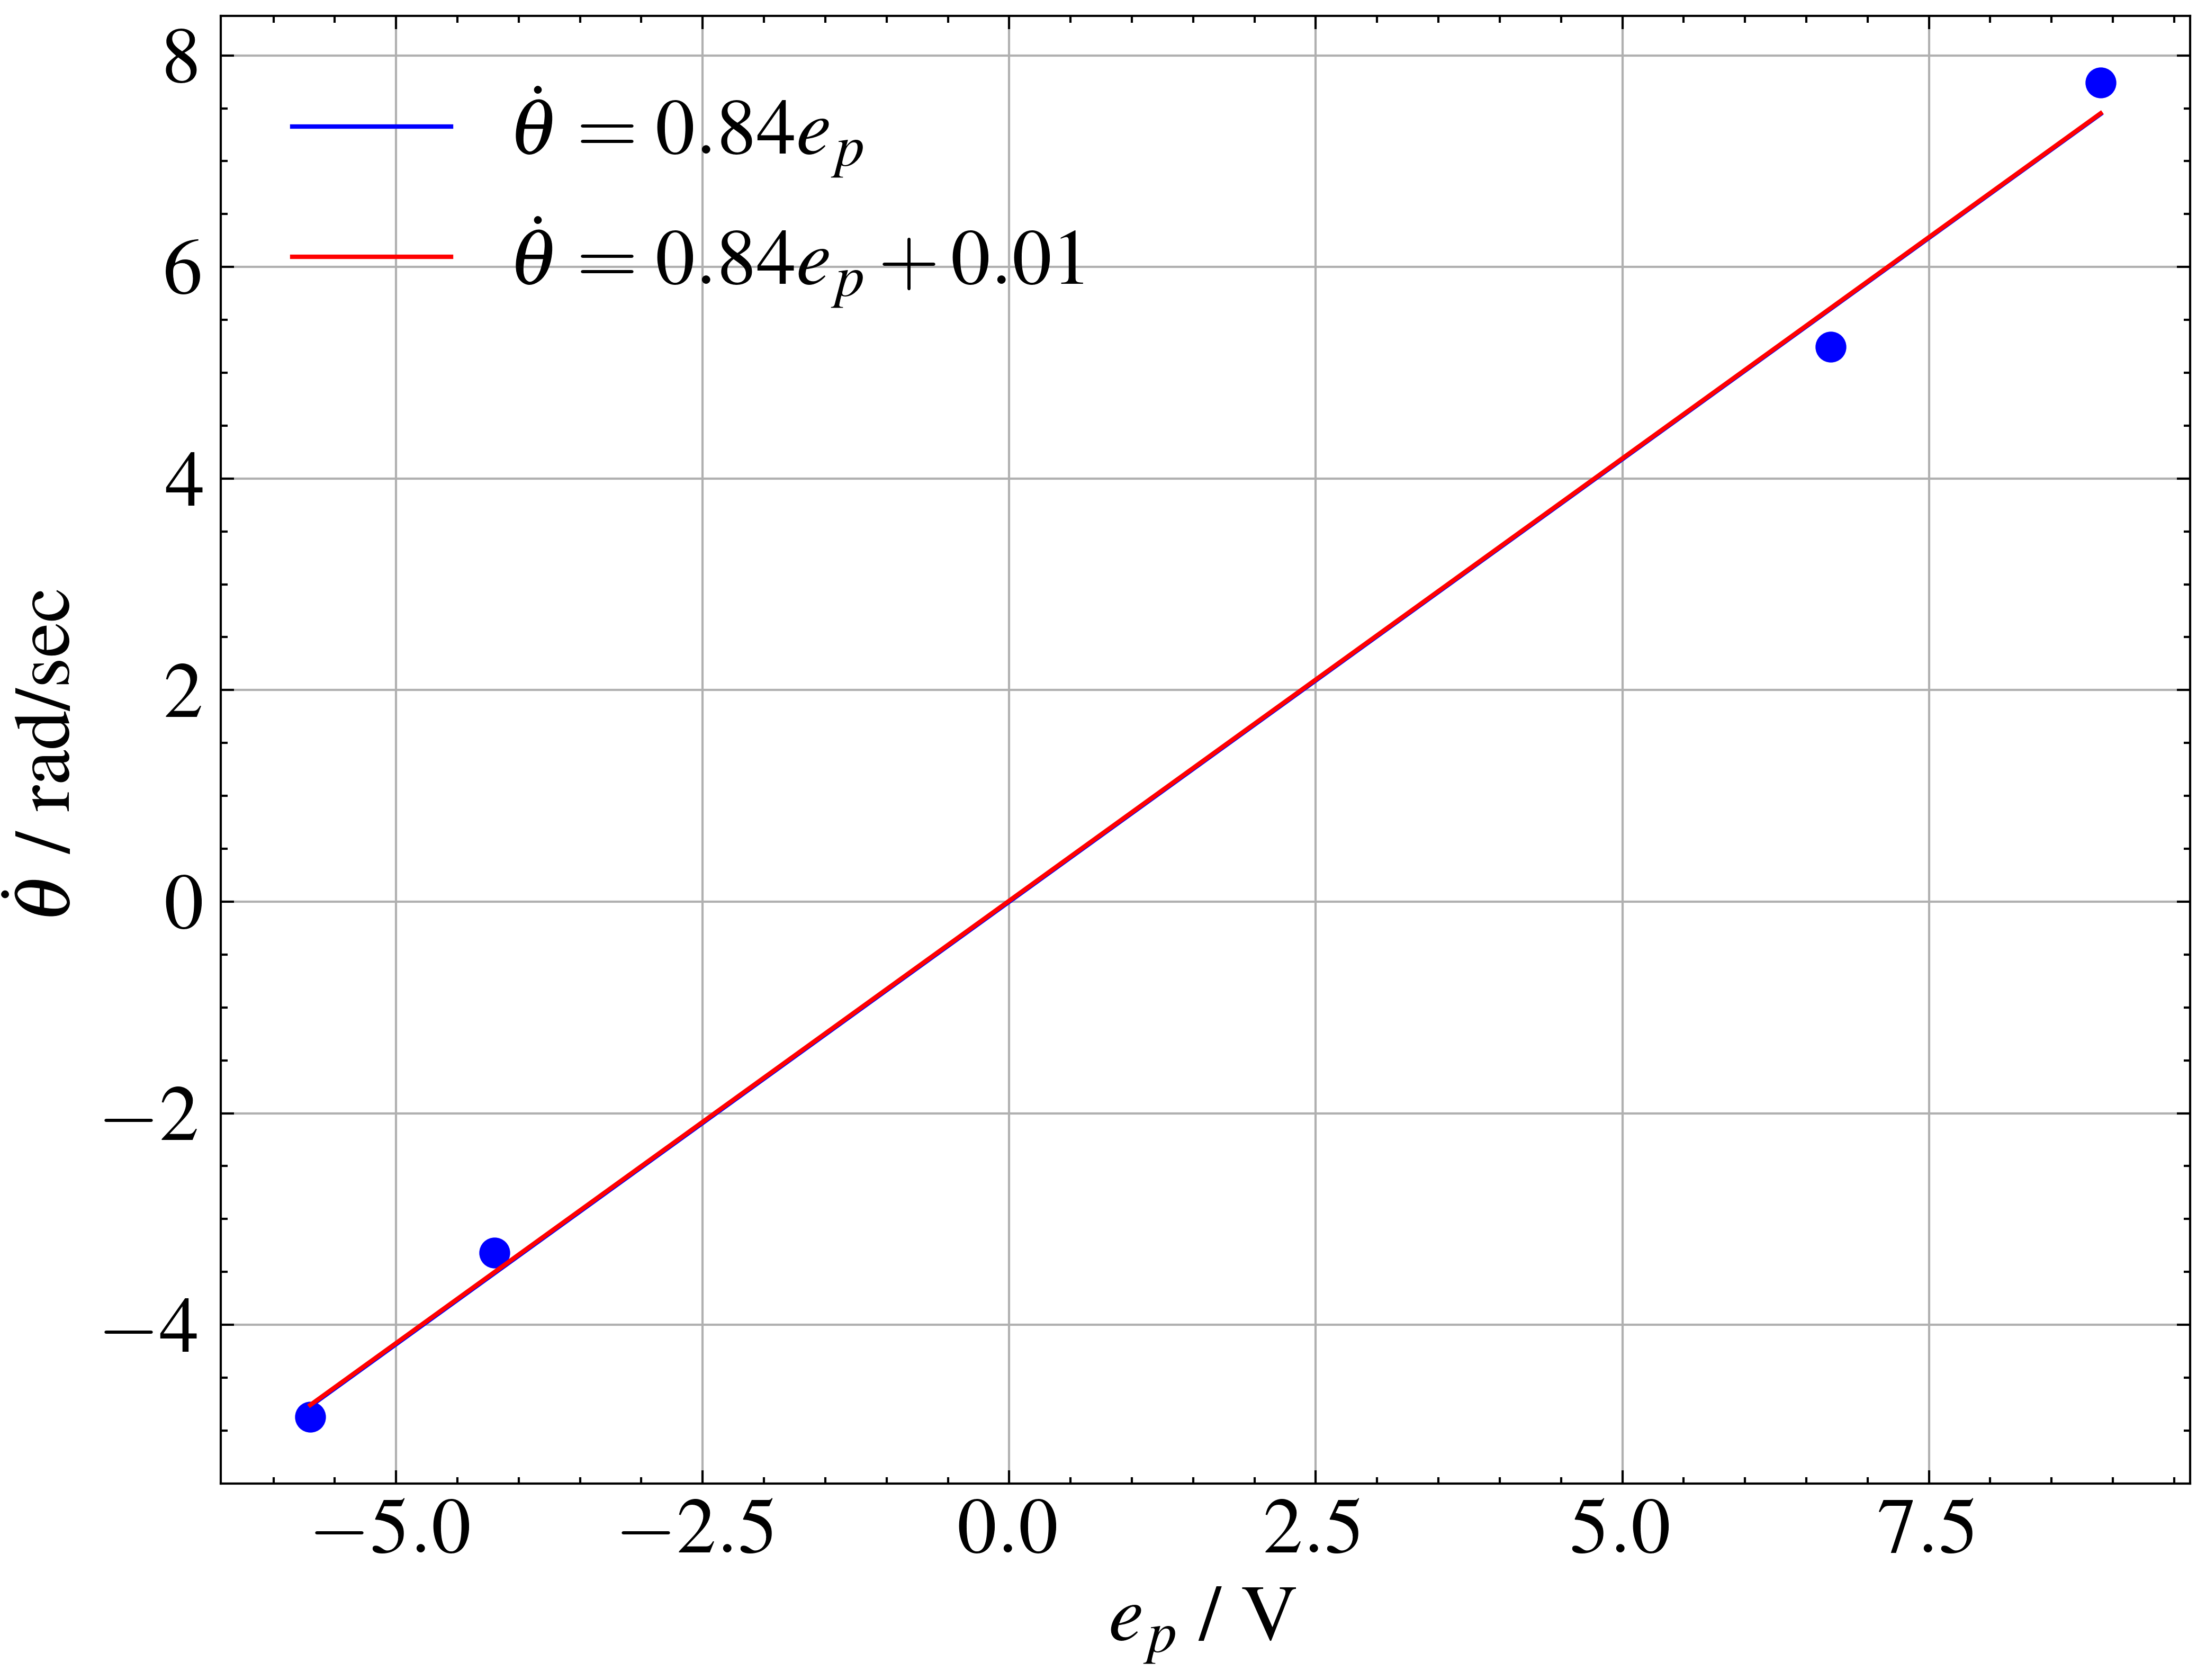
\includegraphics[width=0.8\linewidth]{src/figures/theta_dot-e_p-relation/theta_dot-e_p-relation-P100.png}
		\subcaption{$P=100$}
	\end{subfigure}
	\caption{$P$に対する$e_p$と$\dot{\theta_2}$の関係}\label{fig:theta_dot-e_p-relation}
\end{figure}



最後に、$P$を固定し、$D$を変化させそれに対する$e$, $\dot{\theta_2}$, $e_t$と
$e_t = k \dot{\theta_2}$で計算される$k$の値を表\ref{tab:theta_dot-e_t-relation}に示す。
\begin{table}[!ht]
	\centering
	\begin{tabular}{cccccccc}
		\hline
		$P$ & $D$ & $e$ / \si{\volt} & $\Xi_2$ / rpm & $\dot{\theta_2}$ / rad/s & $e_t$ & $k$ / \si{\volt\sec\per\radian} \\ \hline
		60  & 60  & -1.0             & -220.8        & -5.780                   & -2.8  & 0.4843                          \\
		60  & 60  & -0.8             & -158.9        & -4.159                   & -2.0  & 0.4807                          \\
		60  & 60  & 0.80             & 250           & 6.544                    & 3.4   & 0.5194                          \\
		60  & 60  & 0.40             & 126.8         & 3.319                    & 1.8   & 0.5422                          \\
		60  & 80  & 0.60             & 157.9         & 4.133                    & 3.2   & 0.7741                          \\
		60  & 80  & 0.85             & 237.3         & 6.212                    & 5.3   & 0.8531                          \\
		60  & 80  & -0.8             & -182          & -4.764                   & -3.0  & 0.6296                          \\
		60  & 80  & -0.92            & -220.3        & -5.767                   & -3.8  & 0.6588                          \\
		60  & 100 & -0.94            & -221.9        & -5.809                   & -6.5  & 1.118                           \\
		60  & 100 & -0.78            & -173.3        & -4.536                   & -5.0  & 1.102                           \\
		60  & 100 & 0.58             & 143.6         & 3.759                    & 5.3   & 1.409                           \\
		60  & 100 & 0.98             & 268.1         & 7.018                    & 9.3   & 1.325                           \\ \hline
	\end{tabular}
\end{table}

この表から、$D$に対する$e_t$と$\dot{\theta_2}$の関係を図\ref{fig:theta_dot-e_t-relation}に示す。
\begin{figure}
	\centering
	\begin{subfigure}{0.48\columnwidth}
		\centering
		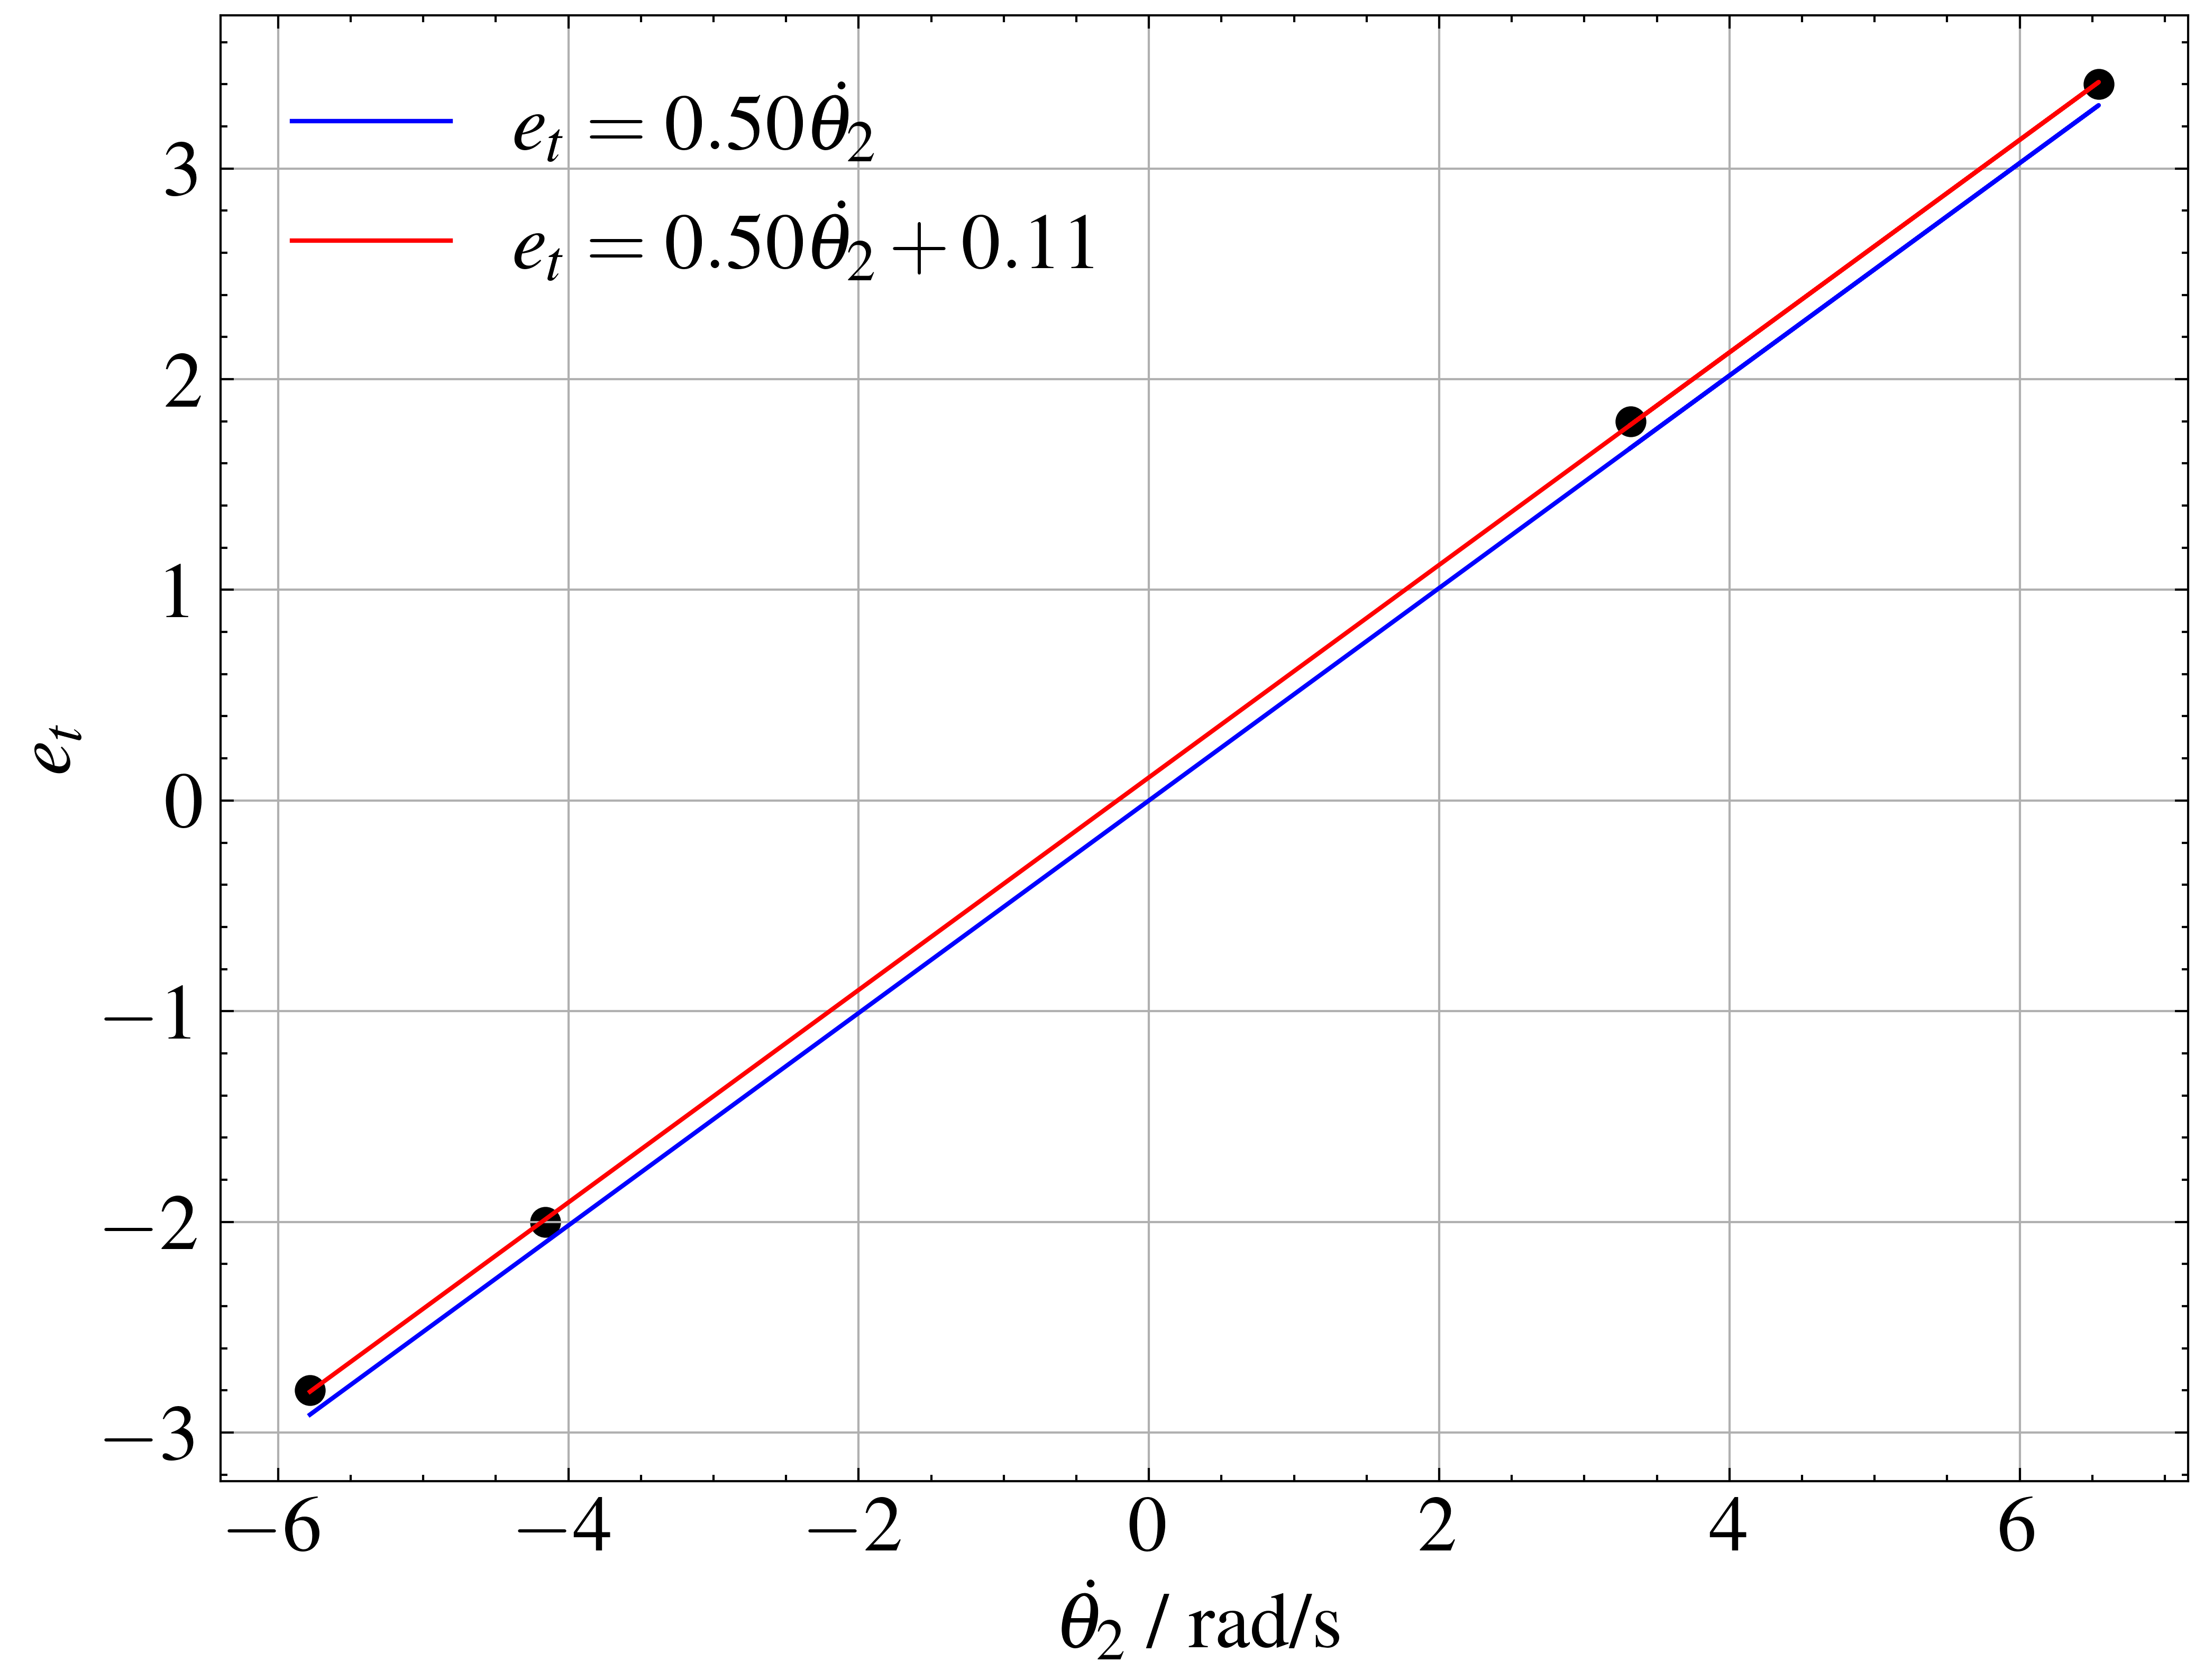
\includegraphics[width=0.8\linewidth]{src/figures/theta_dot-e_t-relation/theta_dot-e_t-relation-D60.png}
		\subcaption{$P=60$}
	\end{subfigure}
	\begin{subfigure}{0.48\columnwidth}
		\centering
		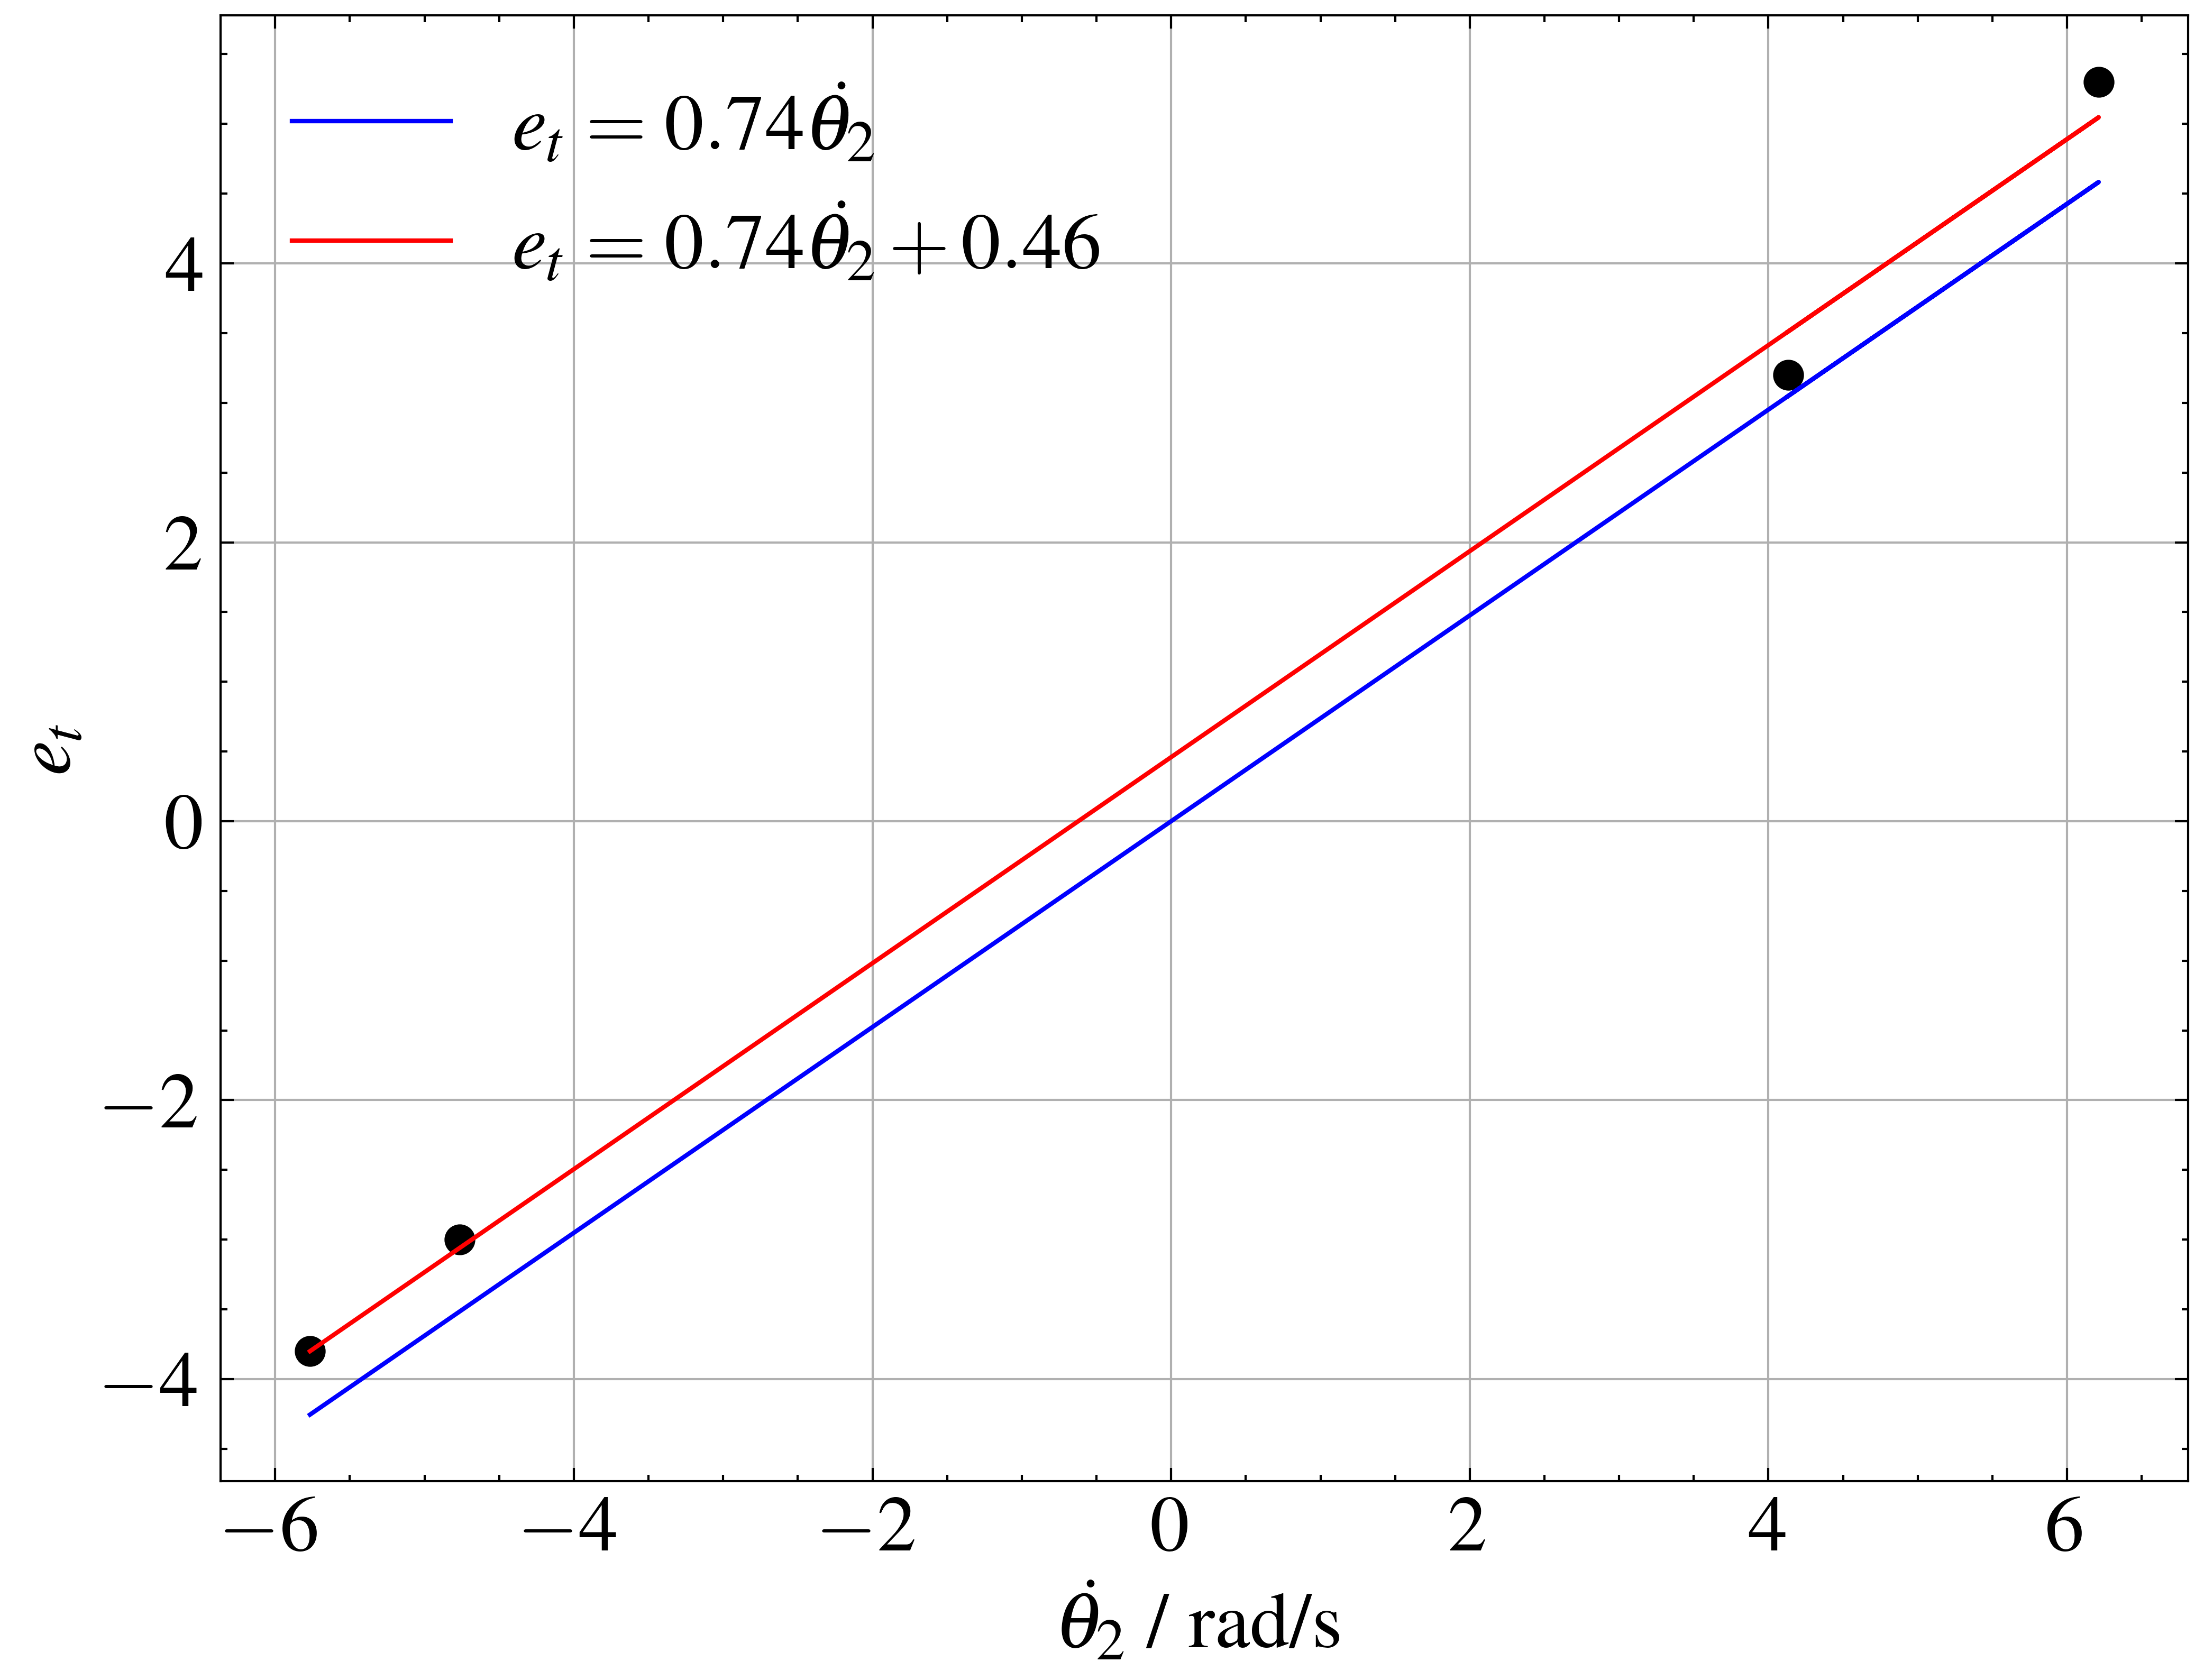
\includegraphics[width=0.8\linewidth]{src/figures/theta_dot-e_t-relation/theta_dot-e_t-relation-D80.png}
		\subcaption{$P=80$}
	\end{subfigure}
	\begin{subfigure}{0.48\columnwidth}
		\centering
		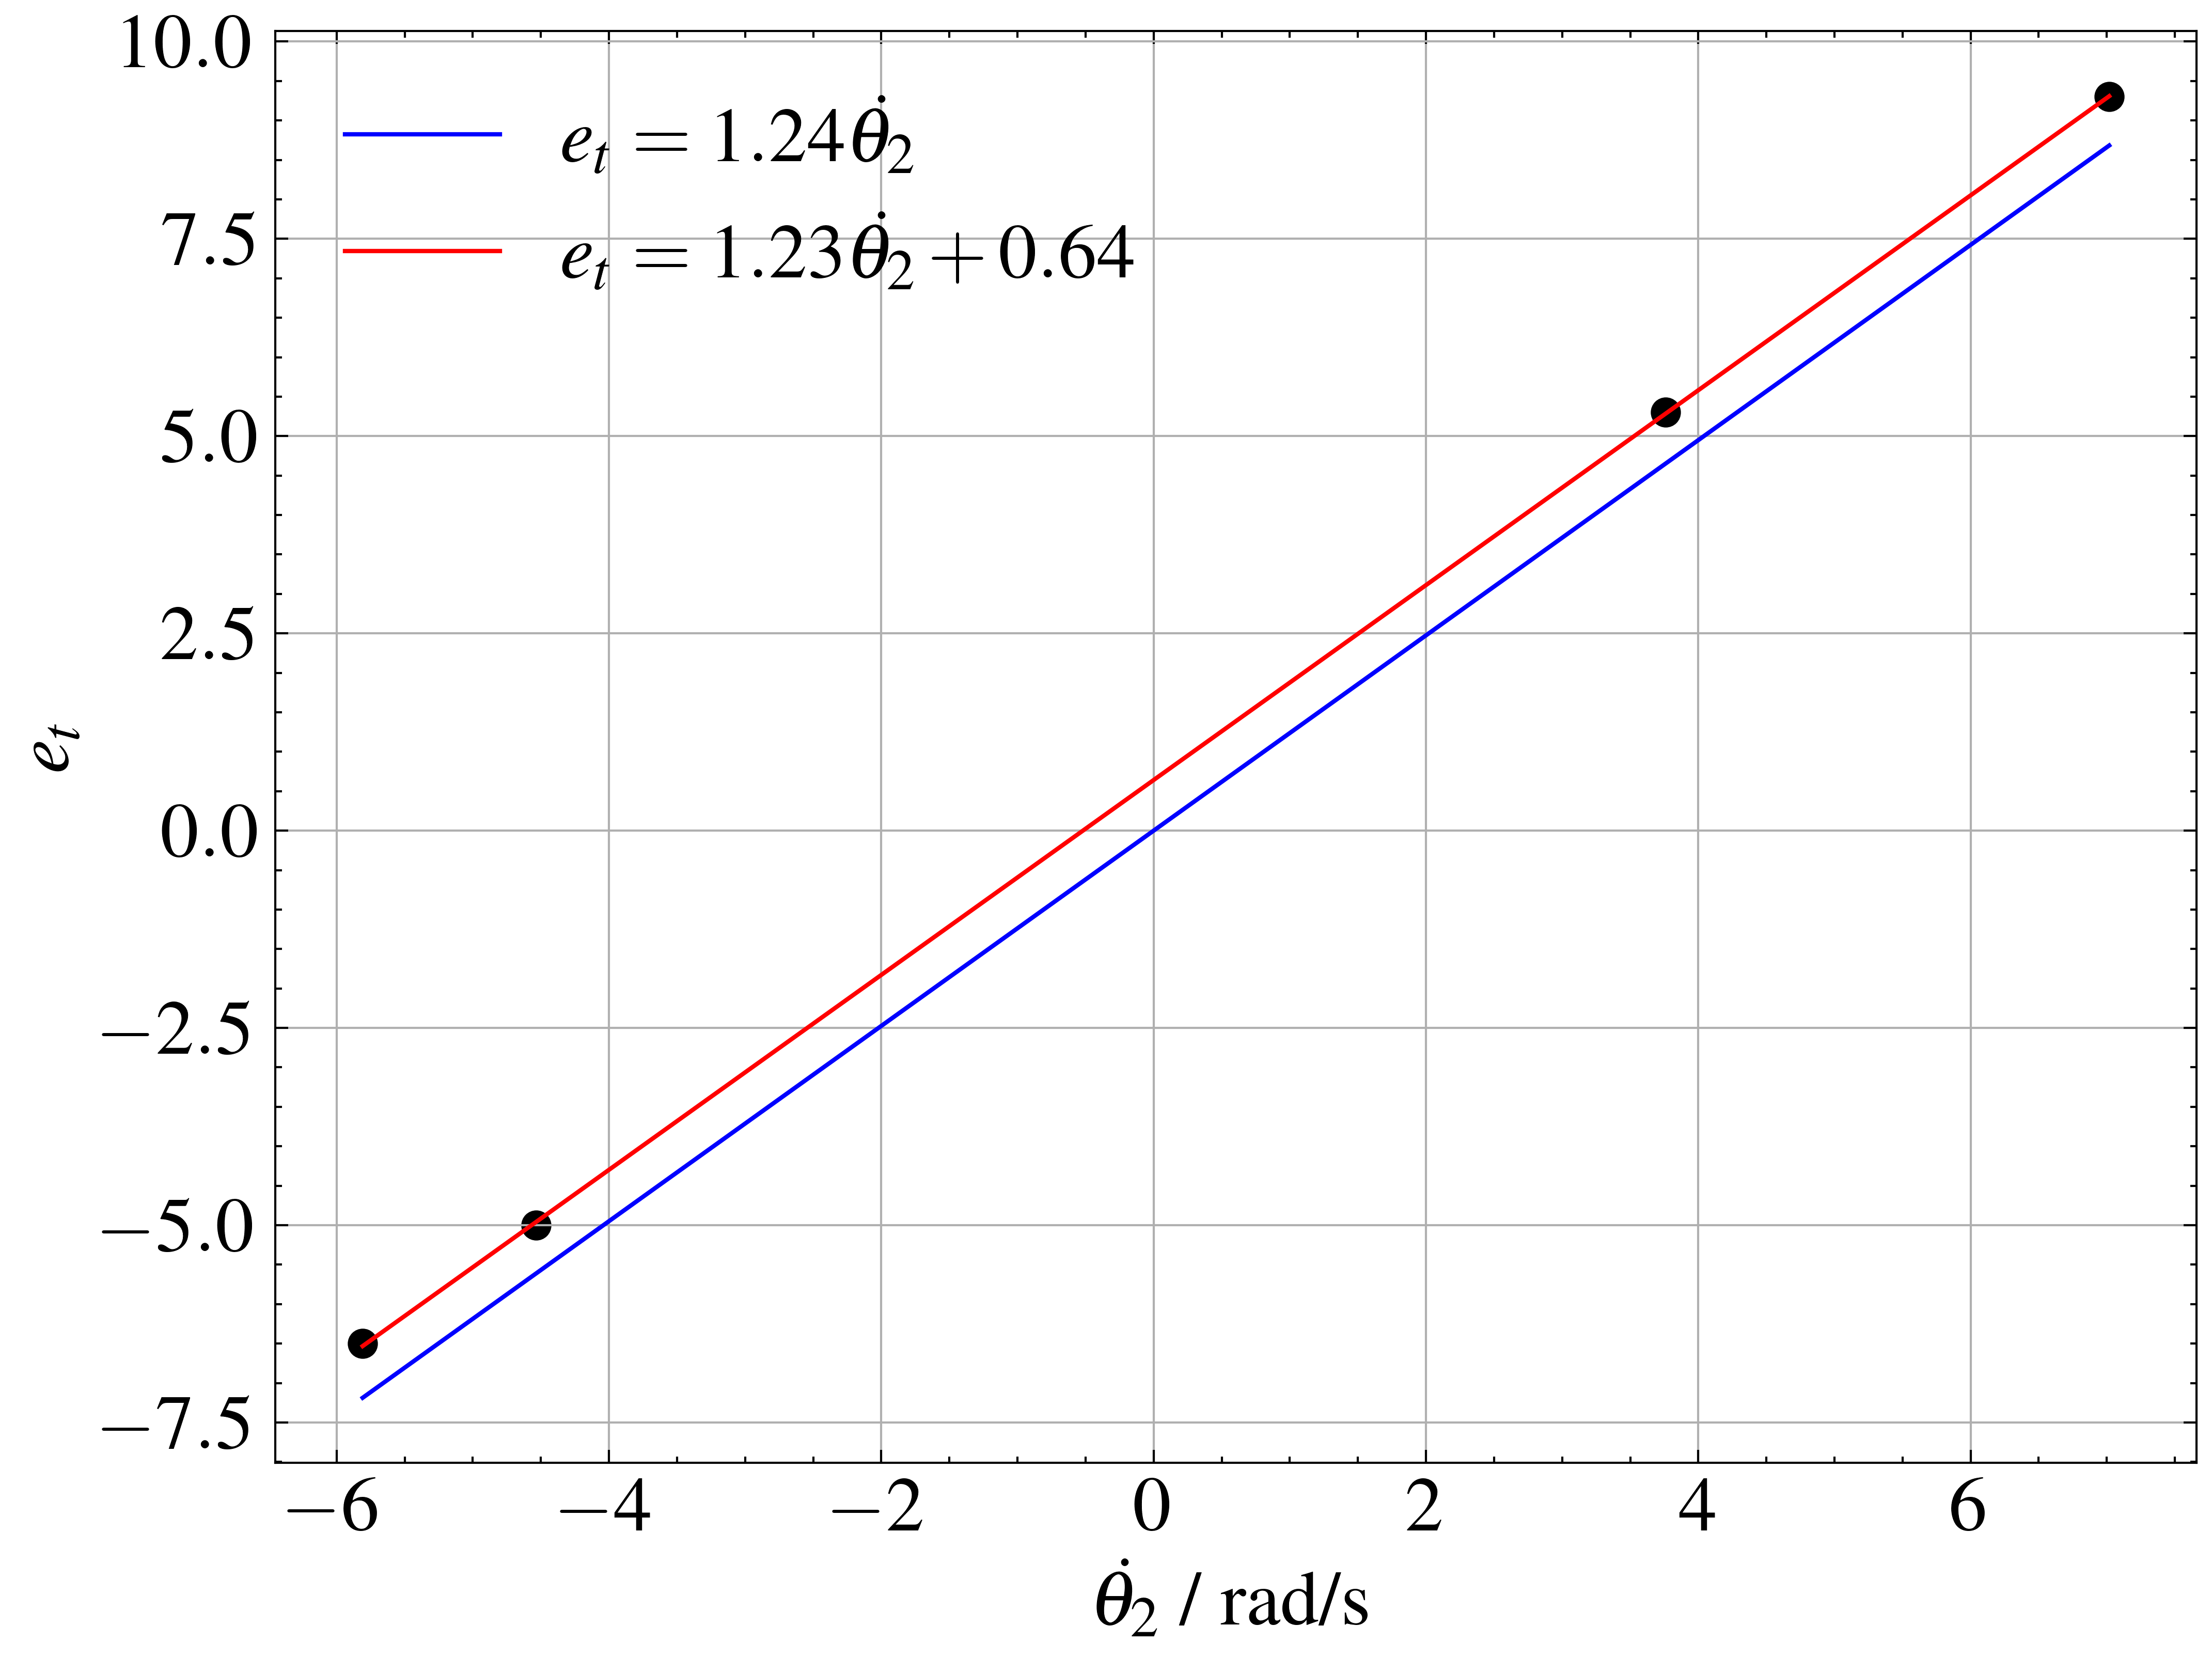
\includegraphics[width=0.8\linewidth]{src/figures/theta_dot-e_t-relation/theta_dot-e_t-relation-D100.png}
		\subcaption{$P=100$}
	\end{subfigure}
	\caption{$D$に対する$e_t$と$\dot{\theta_2}$の関係}\label{fig:theta_dot-e_t-relation}
\end{figure}

これまでと同様に、それぞれ原点を通る直線で近似したものと、一次関数で近似したものを示している。
$k_p$と同様に実験値に近い方として一次関数による近似を採用し、
$D=60$のとき、$e_t = 0.50\dot{\theta_2} + 0.11$
$D=80$のとき、$e_t = 0.74\dot{\theta_2} + 0.46$
$D=100$のとき、$e_t = 1.23\dot{\theta_2} + 0.64$
とする。

\clearpage
\subsection{実験1, 2, 3からの結果}
以上の結果をまとめるともとまったパラメータ次のようになる。
\begin{equation}\label{eq:parameter-result}
    \begin{split}
        k1  & = \SI{0.0668}{\volt\per\radian}       \\
        k2  & = \SI{0.334}{\volt\per\radian}        \\
        T   & = \SI{96}{\milli\sec}                 \\
        K   & = \SI{0.85}{\radian\per\sec\per\volt} \\
        e_p & = \left\{
        \begin{alignedat}{3}
            8.58e + 1.23   & \quad (P=60)  \\
            11.93e + 1.32  & \quad (P=80)  \\
            213.97e + 1.62 & \quad (P=100) \\
        \end{alignedat}
        \right.                                     \\
        e_t & = \left\{
        \begin{alignedat}{3}
            0.50\dot{\theta_2} + 0.11 & \quad (D=60)  \\
            0.74\dot{\theta_2} + 0.46 & \quad (D=80)  \\
            1.23\dot{\theta_2} + 0.64 & \quad (D=100) \\
        \end{alignedat}
        \right.
    \end{split}
\end{equation}
また\ref{eq:characteristic-function-parameters}式、
\ref{eq:characteristic-function2-parameters}式より
実験1の各場合で$\omega$、$\zeta$を求めると、次の表\ref{tab:omega}、\ref{tab:zeta}のようになる。
\begin{table}[ht]
	\centering
	\caption{$P$、$D$に対する$\omega$の値}\label{tab:omega}
	\begin{tabular}{|c|c|c|c|}
		\hline
		\diagbox{D}{P} & 60    & 80    & 100    \\ \hline
		0              & 5.037 & 5.940 & 25.155 \\ \hline
		60             & 5.037 & 5.940 & 25.155 \\ \hline
		80             & 5.037 & 5.940 & 25.155 \\ \hline
		100            & 5.037 & 5.940 & 25.155 \\ \hline
	\end{tabular}
\end{table}

\begin{table}[ht]
	\centering
	\caption{$P$、$D$に対する$\zeta$の値}\label{tab:zeta}
	\begin{tabular}{|c|c|c|c|}
		\hline
		\diagbox{D}{P} & 60    & 80    & 100   \\ \hline
		0              & 1.034 & 0.877 & 0.207 \\ \hline
		60             & 1.473 & 1.250 & 0.295 \\ \hline
		80             & 1.684 & 1.428 & 0.337 \\ \hline
		100            & 2.115 & 1.794 & 0.424 \\ \hline
	\end{tabular}
\end{table}








\end{document}
